\documentclass[12pt,a4paper]{report}
\usepackage[utf8]{inputenc}
\usepackage[vietnamese]{babel}
\usepackage{graphicx}
\usepackage{hyperref}
\usepackage{listings}
\usepackage{xcolor}
\usepackage{minted}
\usepackage{float}
\usepackage{geometry}
\usepackage{anyfontsize}

\geometry{a4paper, margin=2.5cm}

\hypersetup{
    colorlinks=true,
    linkcolor=blue,
    filecolor=magenta,      
    urlcolor=cyan,
    pdftitle={Báo cáo Phân tích Dự án},
    pdfpagemode=FullScreen,
}

\begin{document}

% Title page
\begin{titlepage}
    \centering
    \vspace*{1cm}
    
    \textbf{\Large HỌC VIỆN CÔNG NGHỆ BƯU CHÍNH VIỄN THÔNG}
    
    \textbf{\large KHOA CÔNG NGHỆ THÔNG TIN 1}
    
    \vspace{0.5cm}
    \underline{\hspace{3cm}} o0o \underline{\hspace{3cm}}
    
    \vspace{1cm}
    
\includegraphics[width=0.35\linewidth]{images/ptit_logo.png}
    
    \vspace{1.5cm}
    \textbf{\LARGE BÁO CÁO THỰC TẬP CƠ SỞ}
    \vspace{0.5cm}

    \textbf{\Large VIỆT FOOD - ỨNG DỤNG WEB ĐẶT ĐỒ ĂN VIỆT NAM TÍCH HỢP AI AGENT} 
    \vspace{1cm}

    \author{Lại Xuân Hiếu}

    \begin{tabular}{ll}
        {\textbf{\large Người thực hiện }} & {\textbf{\large Lại Xuân Hiếu}} \\
        {\textbf{\large Giảng Viên Hướng Dẫn }} & {\textbf{\large TS.Dương Trần Đức}} \\
    \end{tabular}

    \vfill
    \today
\end{titlepage}



\tableofcontents

\chapter{Giới thiệu tổng quan}
\section{Giới thiệu dự án}
Việt Food là một ứng dụng web fullstack với kiến trúc client-server nhằm cung cấp nền tảng đặt món ăn Việt Nam trực tuyến. Ứng dụng được phát triển với mục đích tạo ra trải nghiệm người dùng hiện đại, thân thiện, đồng thời đảm bảo hiệu suất cao và khả năng mở rộng. Với giao diện người dùng trực quan và hệ thống backend mạnh mẽ, Việt Food nhằm mục đích kết nối người dùng với các món ăn truyền thống và hiện đại của ẩm thực Việt Nam.

\begin{figure}[H]
    \centering
    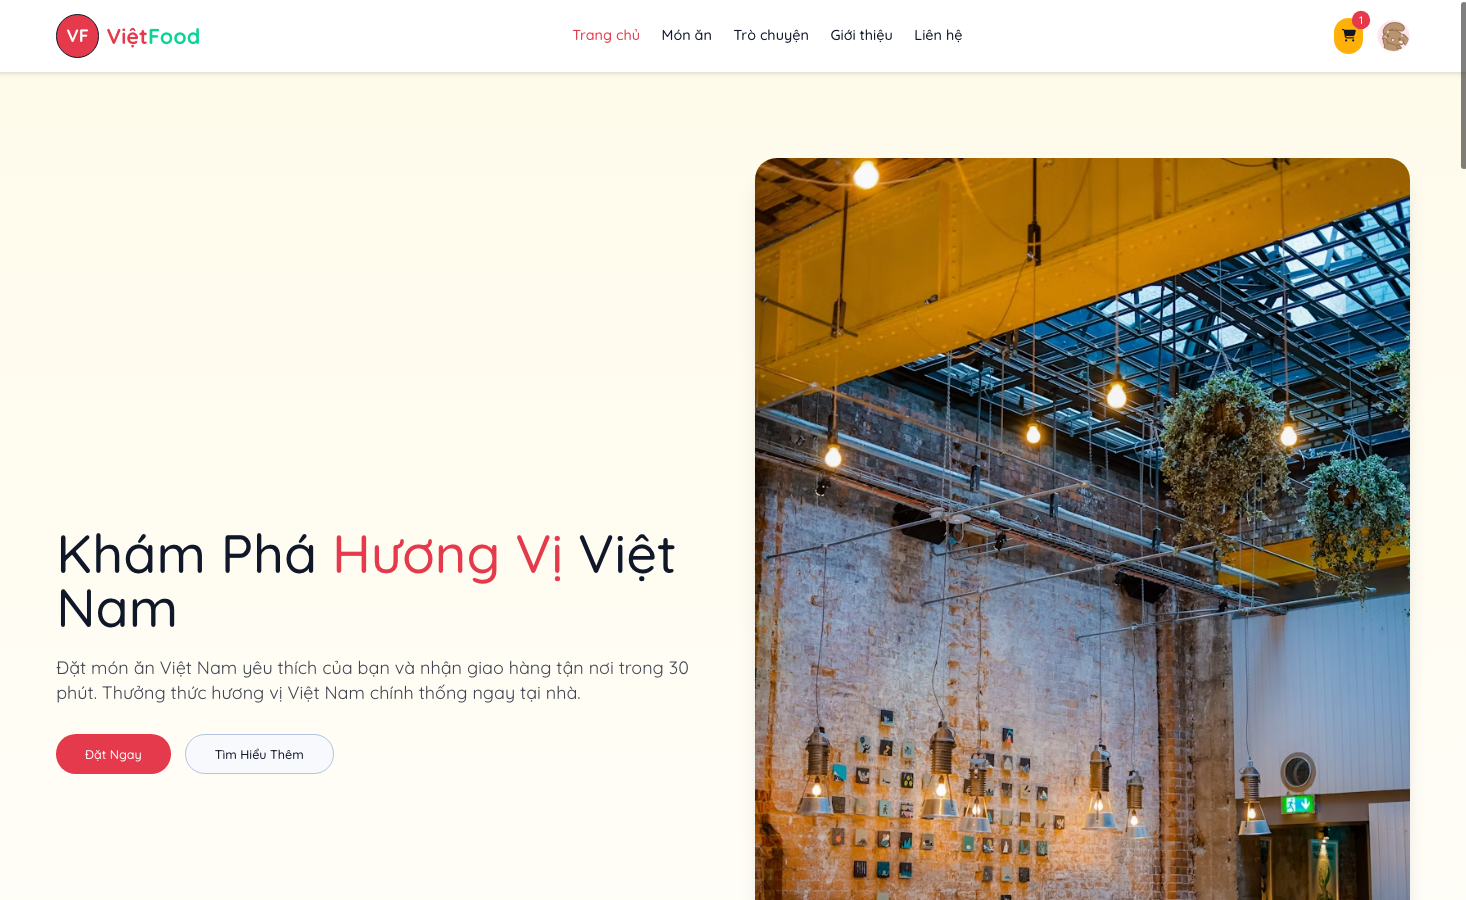
\includegraphics[width=0.9\textwidth]{images/home-page.png}
    \caption{Giao diện trang chủ ứng dụng Việt Food}
    \label{fig:home-page}
\end{figure}

Hình \ref{fig:home-page} thể hiện giao diện chính của ứng dụng, nơi người dùng có thể xem các món ăn nổi bật, tìm kiếm món ăn và dễ dàng đặt hàng.

\begin{figure}[H]
    \centering
    \begin{minipage}{0.48\textwidth}
        \centering
        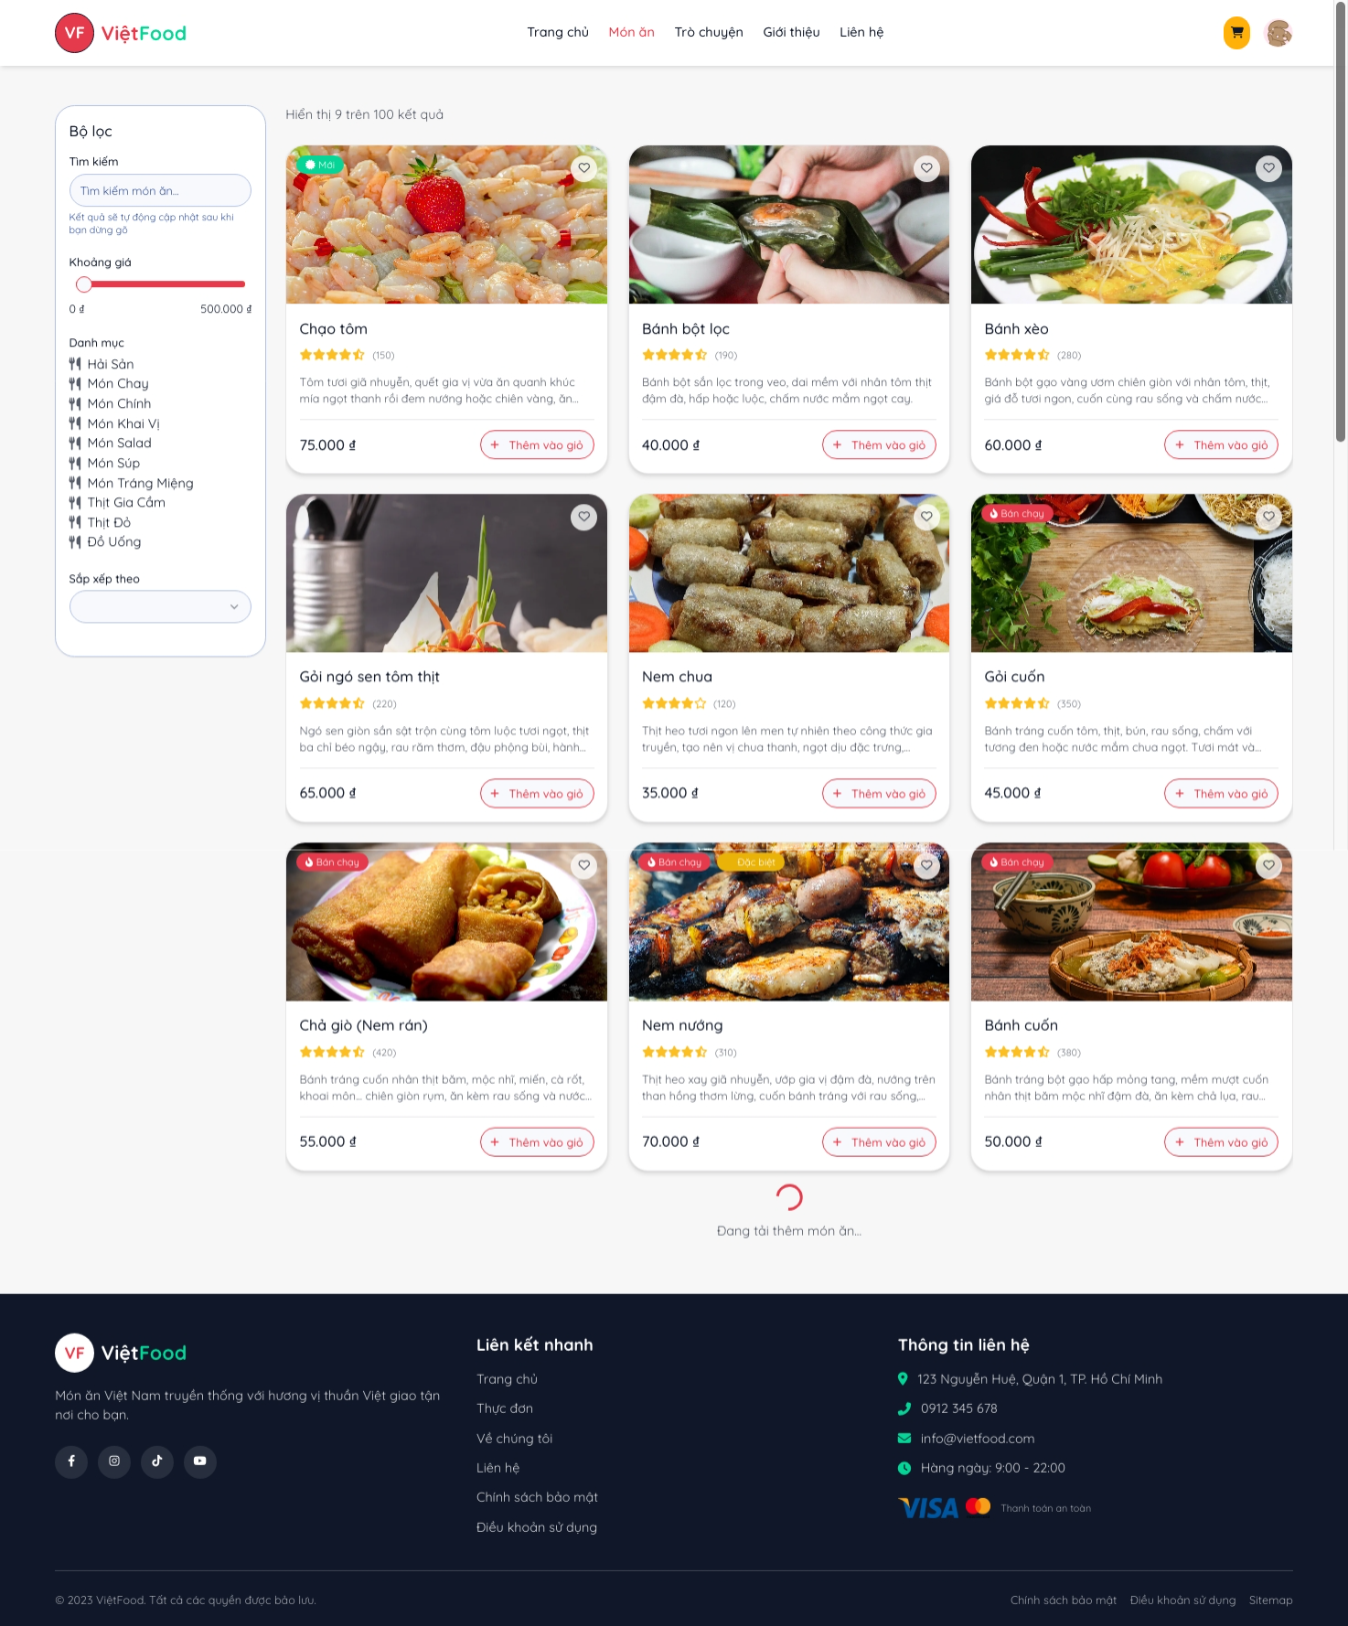
\includegraphics[width=\textwidth]{images/shopping-page.png}
        \caption{Trang đặt món ăn}
        \label{fig:shopping}
    \end{minipage}
    \hfill
    \begin{minipage}{0.48\textwidth}
        \centering
        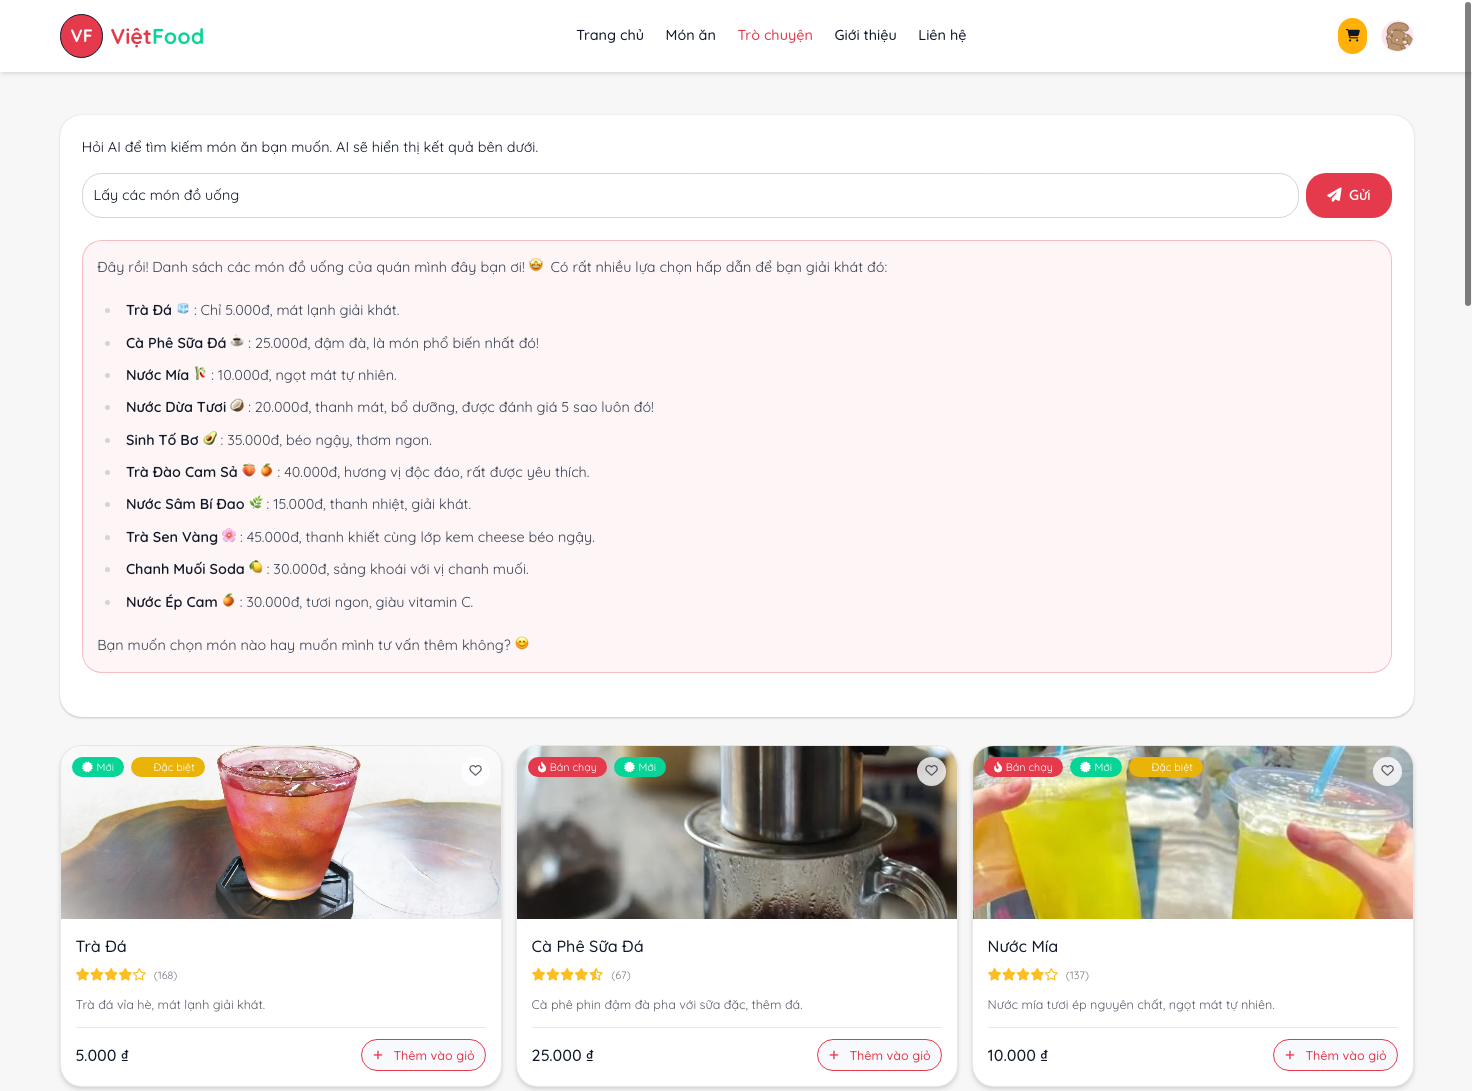
\includegraphics[width=\textwidth]{images/chat-page.png}
        \caption{Tính năng chat hỗ trợ}
        \label{fig:chat}
    \end{minipage}
\end{figure}

\begin{figure}[H]
    \centering
    \begin{minipage}{0.48\textwidth}
        \centering
        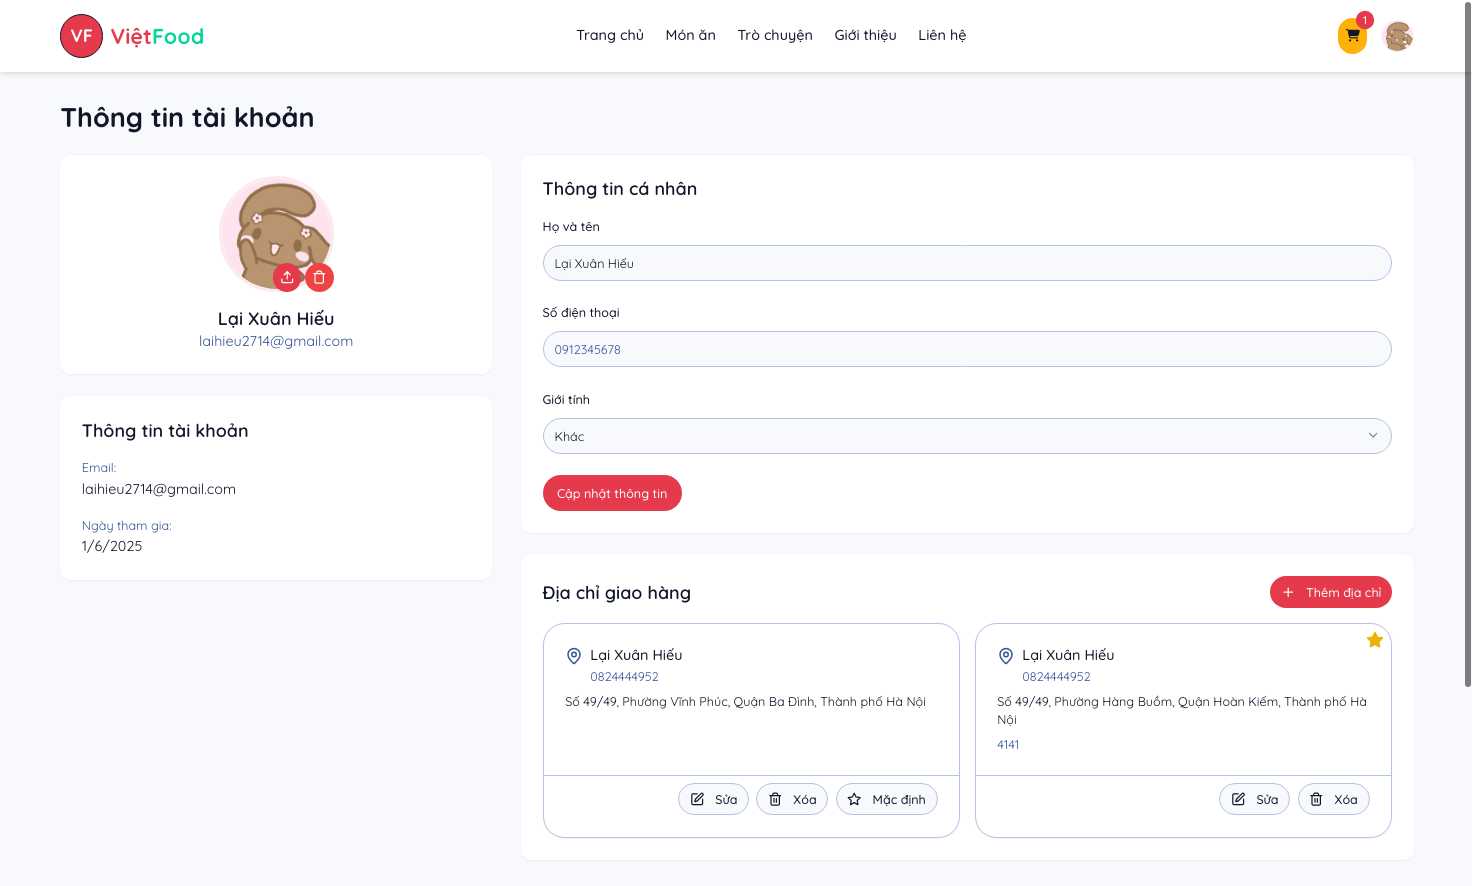
\includegraphics[width=\textwidth]{images/profile-page.png}
        \caption{Trang thông tin cá nhân}
        \label{fig:profile}
    \end{minipage}
    \hfill
    \begin{minipage}{0.48\textwidth}
        \centering
        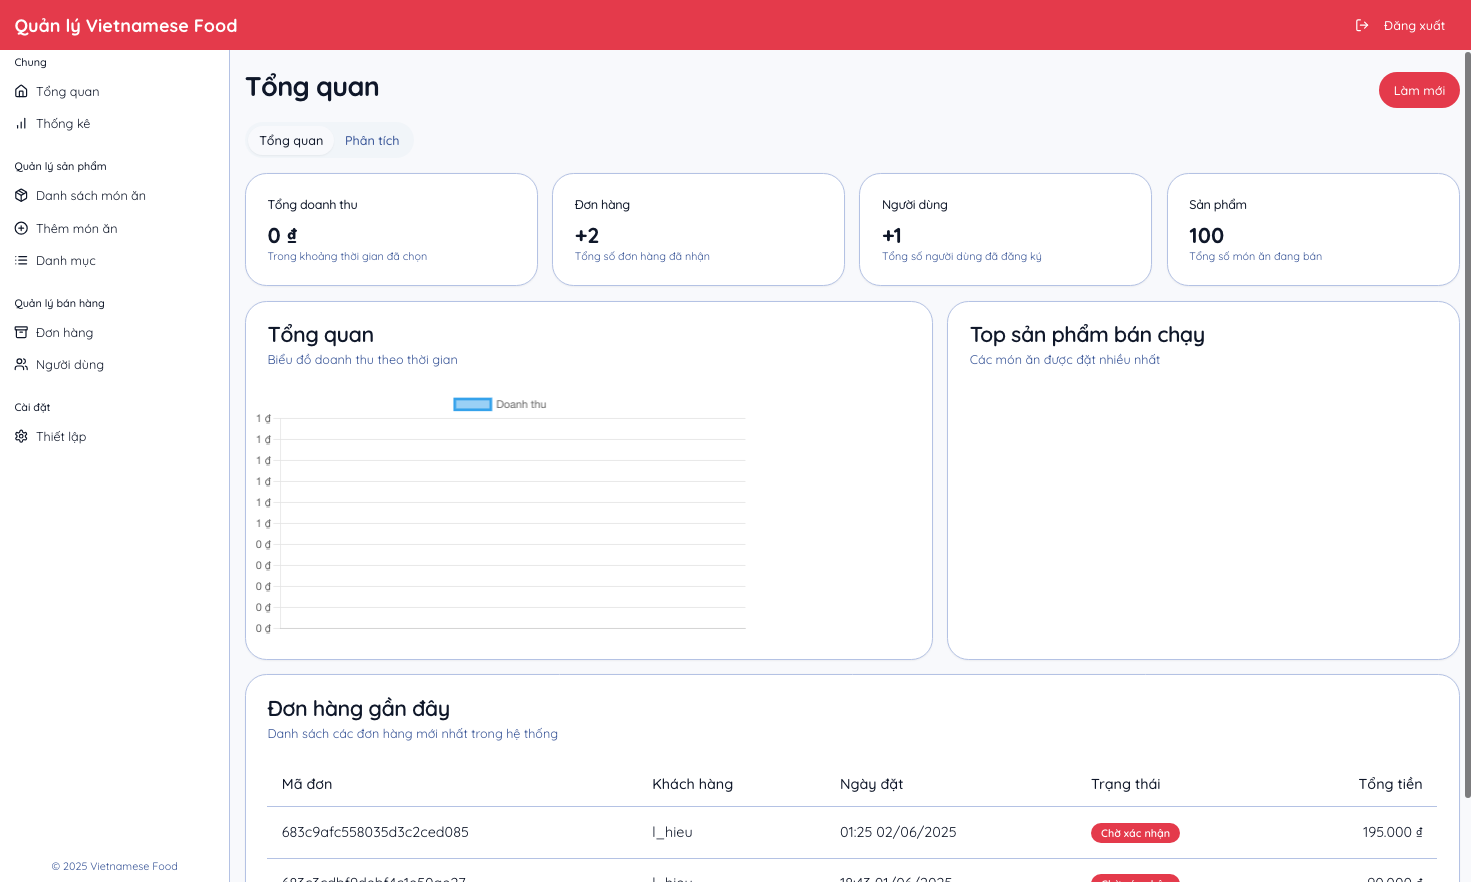
\includegraphics[width=\textwidth]{images/admin-page.png}
        {\footnotesize \caption{Trang quản trị viên}}
        \label{fig:admin}
    \end{minipage}
\end{figure}

\section{Công nghệ sử dụng}
Dự án được xây dựng bằng các công nghệ hiện đại:

\subsection{Backend}
\begin{itemize}
    \item \textbf{Node.js} và \textbf{Express}: Framework cho phát triển ứng dụng web server-side.
    \item \textbf{TypeScript}: Ngôn ngữ lập trình đảm bảo tính mạnh mẽ và an toàn cho mã nguồn.
    \item \textbf{MongoDB}: Cơ sở dữ liệu NoSQL phục vụ lưu trữ dữ liệu phi quan hệ.
    \item \textbf{Redis}: Hệ thống cache bộ nhớ để tối ưu hóa hiệu suất truy vấn.
    \item \textbf{Redis Stream}: Xử lý các tin nhắn và sự kiện real-time.
    \item \textbf{Compression}: Middleware giảm kích thước phản hồi HTTP.
    \item \textbf{Sharp}: Thư viện xử lý và tối ưu hóa hình ảnh.
    \item \textbf{Elasticsearch}: Công cụ tìm kiếm và đánh chỉ mục dữ liệu nhanh chóng.
    \item \textbf{Gemini AI}: Tích hợp trí tuệ nhân tạo cho các tính năng thông minh.
\end{itemize}

\subsection{Frontend}
\begin{itemize}
    \item \textbf{React}: Thư viện JavaScript để xây dựng giao diện người dùng tương tác.
    \item \textbf{TypeScript}: Đảm bảo type safety và khả năng bảo trì cho mã nguồn frontend.
    \item \textbf{Tailwind CSS}: Framework CSS tiện ích giúp phát triển UI nhanh chóng và đồng nhất.
    \item \textbf{React Hook Form}: Quản lý biểu mẫu với hiệu suất cao.
    \item \textbf{Zod}: Thư viện xác thực dữ liệu với TypeScript.
\end{itemize}

\chapter{Phân tích kiến trúc và thiết kế hệ thống}
\section{Kiến trúc tổng thể}

Việt Food áp dụng kiến trúc client-server hiện đại, với sự phân chia rõ ràng giữa frontend (React) và backend (Node.js/Express). Kiến trúc này tạo nên một hệ thống linh hoạt và mạnh mẽ, mang lại nhiều lợi ích:

\begin{itemize}
    \item \textbf{Phát triển độc lập}:
    \item \textbf{Khả năng mở rộng}
    \item \textbf{Tái sử dụng API}
    \item \textbf{Bảo mật tốt hơn}
    \item \textbf{Hiệu suất tối ưu}
\end{itemize}

\subsection{Mô hình kiến trúc}
Hệ thống áp dụng kiến trúc MVC (Model-View-Controller) kết hợp với các dịch vụ (Services):

\begin{itemize}
    \item \textbf{Model}: Đại diện cho cấu trúc dữ liệu và xử lý logic liên quan đến dữ liệu.
    \item \textbf{View}: Được thực hiện ở phía client, hiển thị thông tin cho người dùng.
    \item \textbf{Controller}: Xử lý các yêu cầu từ client, tương tác với các service và trả về kết quả.
    \item \textbf{Service}: Chứa logic nghiệp vụ, tương tác với database và các thành phần bên ngoài.
\end{itemize}

\subsection{Sơ đồ kiến trúc}
Kiến trúc hệ thống được thiết kế với nhiều lớp:
% add image here
\begin{figure}[H]
\centering  
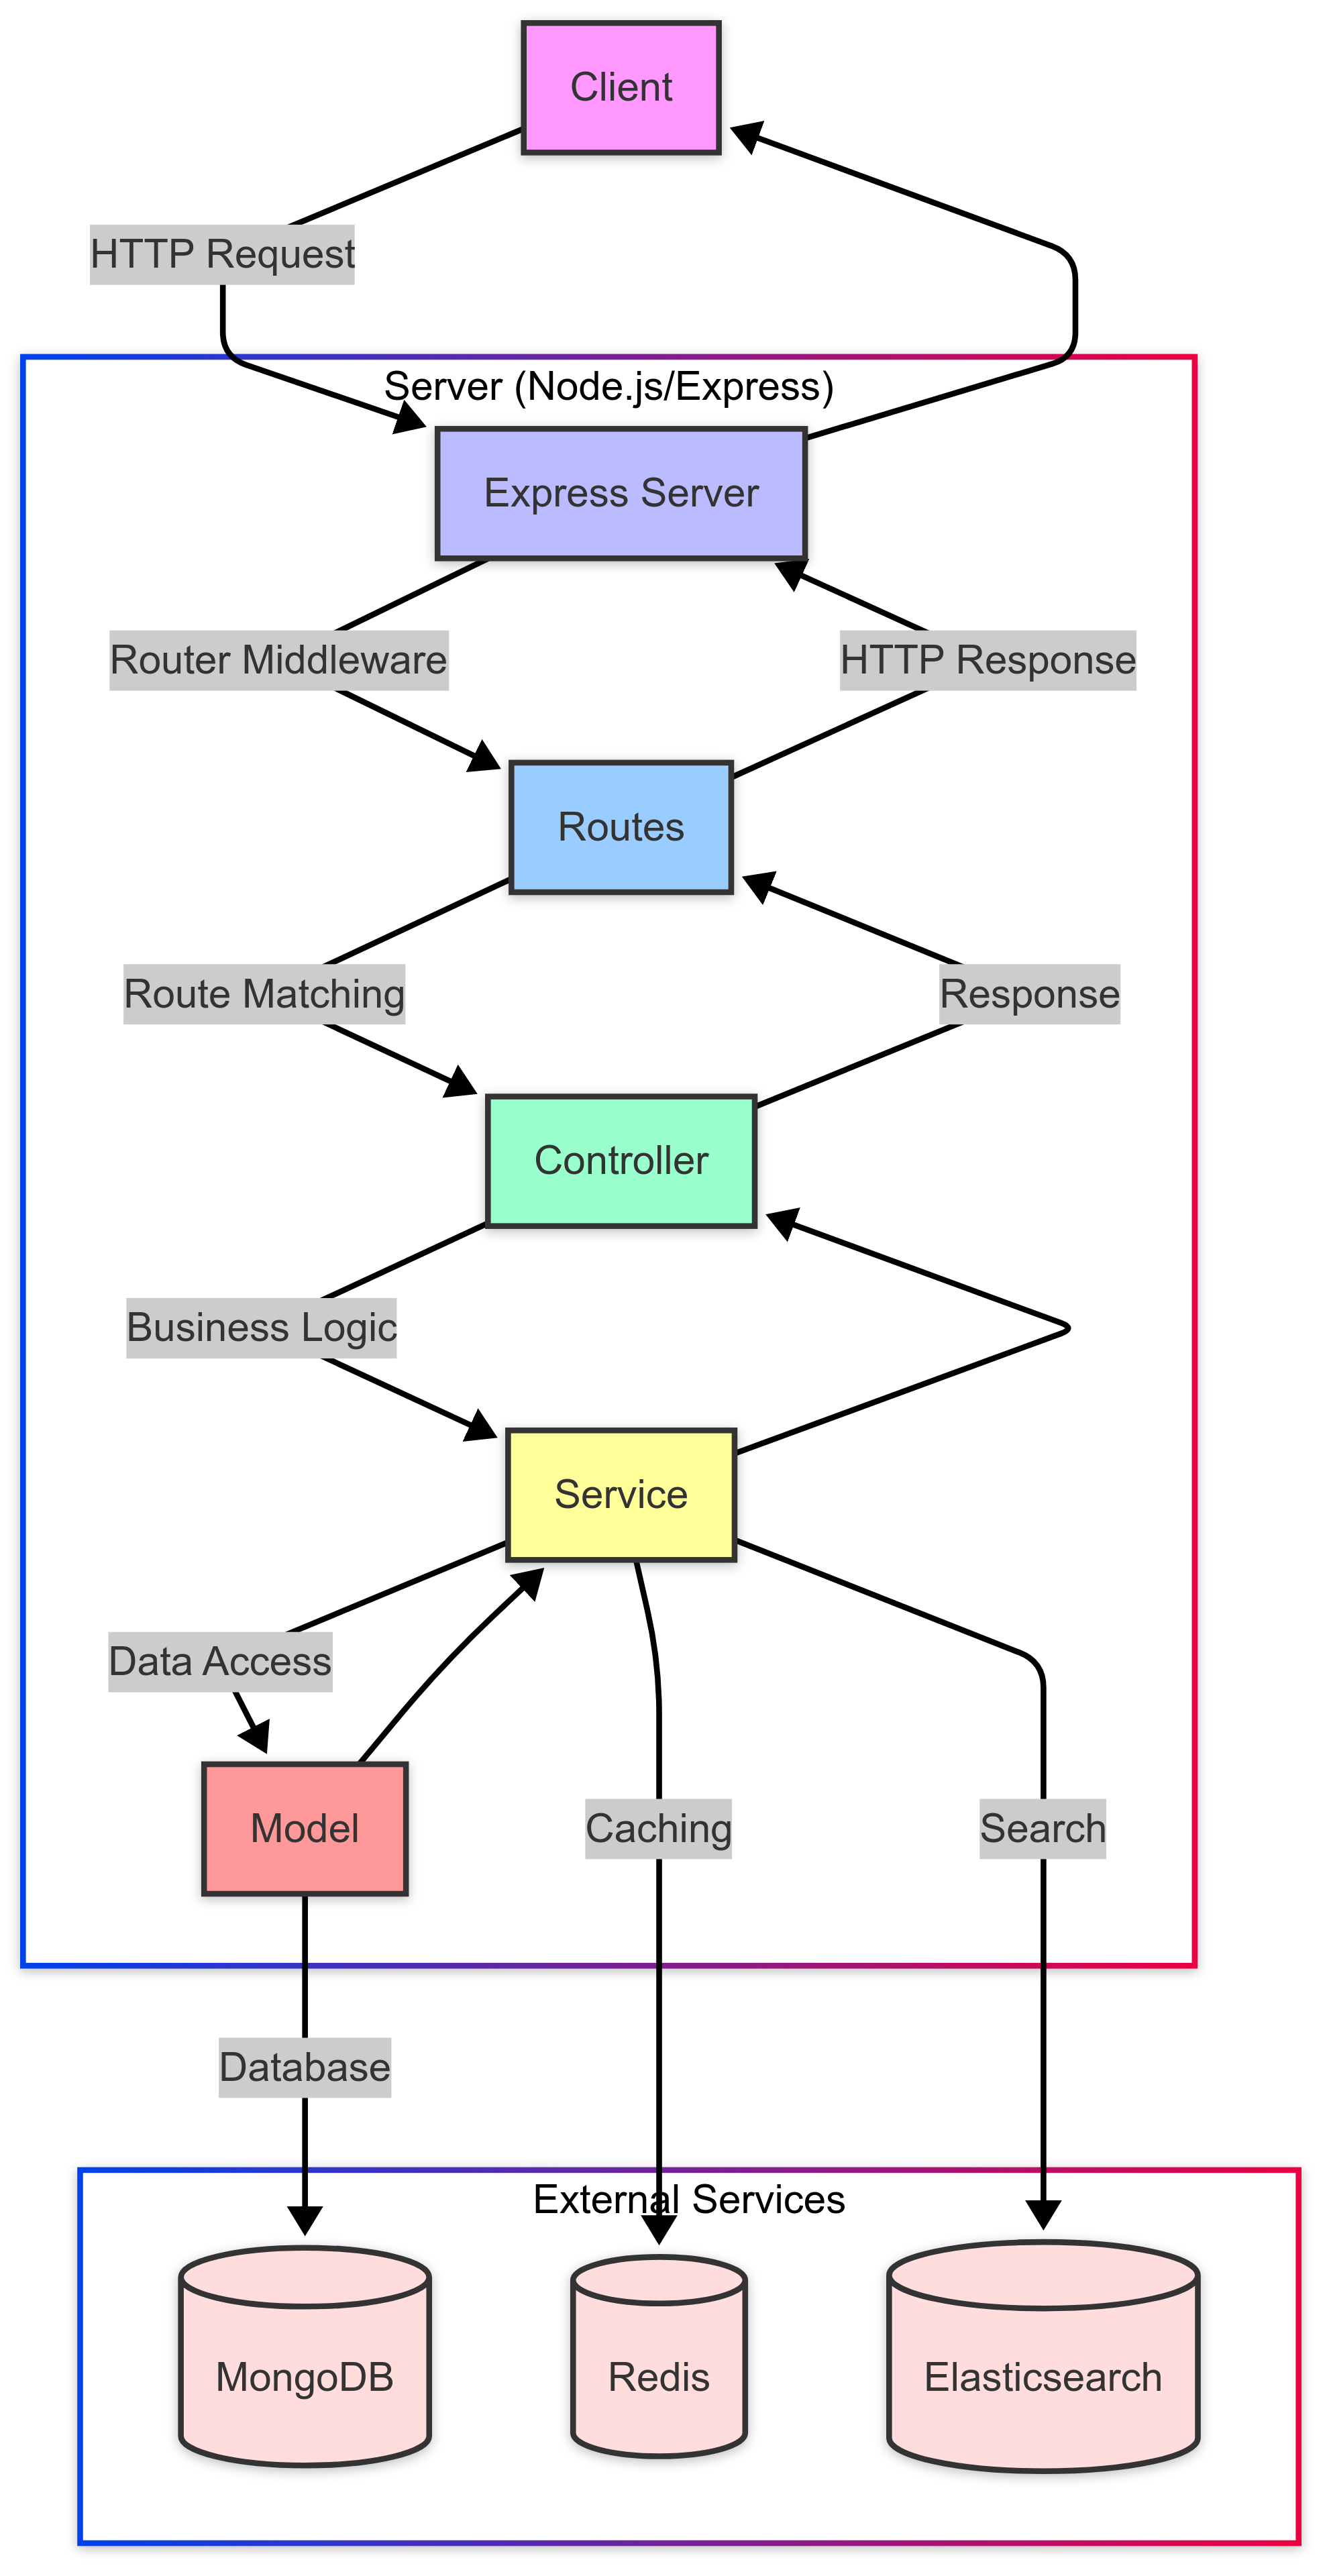
\includegraphics[width=0.8\textwidth]{images/architecture.png}
\caption{Sơ đồ kiến trúc tổng thể của hệ thống Việt Food}
\end{figure}


\section{Thiết kế module/component chính}
Cấu trúc dự án được tổ chức thành các module chức năng riêng biệt, gồm cả phần frontend và backend:

\subsection{Controllers}
Xử lý các request từ client và điều phối các thao tác:
\begin{itemize}
    \item \textbf{DishController}: Quản lý thông tin món ăn
    \item \textbf{CategoryController}: Quản lý danh mục
    \item \textbf{AuthController}: Xử lý xác thực người dùng
    \item \textbf{OrderController}: Xử lý đơn hàng
    \item \textbf{PaymentController}: Xử lý thanh toán
    \item \textbf{UserController}: Xử lý thông tin người dùng
    \item \textbf{UserProfileController}: Xử lý thông tin cá nhân
    \item \textbf{AgentController}: Xử lý tin nhắn chat
    \item \textbf{DashboardController}: Xử lý thống kê
\end{itemize}

\subsection{Services}
Chứa logic nghiệp vụ chính:
\begin{itemize}
    \item \textbf{DishService}: Xử lý logic liên quan đến món ăn, bao gồm caching với Redis
    \item \textbf{CategoryService}: Quản lý danh mục món ăn
    \item \textbf{AuthService}: Xử lý đăng nhập, đăng ký và xác thực
    \item \textbf{SearchService}: Tương tác với Elasticsearch để tìm kiếm
    \item \textbf{PaymentService}: Xử lý thanh toán
    \item \textbf{OrderService}: Xử lý đơn hàng
    \item \textbf{UserService}: Xử lý thông tin người dùng
    \item \textbf{AgentService}: Xử lý tin nhắn chat
    \item \textbf{DashboardService}: Xử lý thống kê
    \item \textbf{MessageWorkerService}: Xử lý tin nhắn với Redis Stream
    \item \textbf{MessageService}: Xử lý tin nhắn
\end{itemize}

\subsection{Middlewares}
Xử lý các tác vụ trung gian:
\begin{itemize}
    \item \textbf{Authentication}: Kiểm tra và xác thực người dùng
    \item \textbf{ImageProcessor}: Xử lý và tối ưu hóa hình ảnh với Sharp
\end{itemize}

\subsection{Models}
Mô tả cấu trúc dữ liệu chính trong backend:
\begin{itemize}
    \item \textbf{DishModel}: Mô hình dữ liệu cho món ăn
    \item \textbf{CategoryModel}: Mô hình dữ liệu cho danh mục
    \item \textbf{UserModel}: Mô hình dữ liệu người dùng
    \item \textbf{MessageModel}: Mô hình dữ liệu tin nhắn
    \item \textbf{OrderModel}: Mô hình dữ liệu đơn hàng
    \item \textbf{PaymentModel}: Mô hình dữ liệu thanh toán
\end{itemize}

\subsection{Frontend Components}
Frontend được xây dựng theo kiến trúc component-based với React, tổ chức thành các thành phần:
\begin{itemize}
    \item \textbf{UI Components}: Các component giao diện cơ bản, được xây dựng trên Radix UI và tùy chỉnh với Tailwind CSS
    \item \textbf{Layout Components}: Quản lý bố cục chung của ứng dụng
    \item \textbf{Page Components}: Tương ứng với các trang trong ứng dụng
\end{itemize}

\subsection{Frontend Services và Hooks}
Phần frontend sử dụng các service và custom hooks để quản lý logic:
\begin{itemize}
    \item \textbf{API Services}: Xử lý các tương tác với backend thông qua axios
    \item \textbf{Context API}: Sử dụng React Context để quản lý trạng thái toàn cục như xác thực người dùng (CartContext, AuthContext)
    \item \textbf{Custom Hooks}: Các hooks chuyên biệt như useAuth, useCart, useProfile để đơn giản hóa quản lý trạng thái và data fetching
    \item \textbf{Local Storage}: Lưu trữ tokens xác thực và thông tin session người dùng
\end{itemize}

\subsection{Quản lý Routing}
Việt Food sử dụng thư viện wouter để quản lý routing trong ứng dụng, với các route chính:
\begin{itemize}
    \item \textbf{Public Routes}: Trang chủ, danh sách món ăn, chi tiết món ăn, tìm kiếm
    \item \textbf{Protected Routes}: Giỏ hàng, quản lý đơn hàng, tài khoản cá nhân
    \item \textbf{Admin Routes}: Quản lý món ăn, danh mục, người dùng và thống kê
\end{itemize}

\subsection{State Management}
Quản lý trạng thái trong ứng dụng được thực hiện thông qua:
\begin{itemize}
    \item \textbf{React Context}: Quản lý trạng thái toàn cục như thông tin người dùng, giỏ hàng
    \item \textbf{Local Component State}: Quản lý trạng thái độc lập của từng component
\end{itemize}

\section{Thiết kế cơ sở dữ liệu}
Hệ thống sử dụng MongoDB làm cơ sở dữ liệu chính với thiết kế schema linh hoạt, phù hợp với đặc thù của ứng dụng đặt đồ ăn. Các collection chính được thiết kế như sau:

\subsection{Các collection chính}
\begin{itemize}
    \item \textbf{Users}: Quản lý thông tin người dùng
    \begin{itemize}
        \item \texttt{username}, \texttt{email}: Thông tin đăng nhập (duy nhất)
        \item \texttt{password}: Mật khẩu đã được mã hóa
        \item \texttt{role}: Phân quyền người dùng (USER/ADMIN)
        \item \texttt{isActive}: Trạng thái tài khoản
    \end{itemize}
    
    \item \textbf{Dishes}: Quản lý thông tin món ăn
    \begin{itemize}
        \item \texttt{name}, \texttt{description}: Thông tin cơ bản
        \item \texttt{price}, \texttt{imageUrl}: Giá và hình ảnh
        \item \texttt{category}: Tham chiếu đến danh mục
        \item \texttt{rating}, \texttt{soldCount}: Đánh giá và số lượng bán
        \item \texttt{isAvailable}, \texttt{isPopular}, \texttt{isNewDish}, \texttt{isSpecial}: Các cờ trạng thái
    \end{itemize}
    
    \item \textbf{Orders}: Quản lý đơn hàng
    \begin{itemize}
        \item \texttt{userId}: Người đặt hàng
        \item \texttt{orderItems}: Danh sách món đã đặt
        \item \texttt{totalAmount}: Tổng tiền
        \item \texttt{status}: Trạng thái đơn hàng
        \item \texttt{address}: Thông tin giao hàng
    \end{itemize}
    
    \item \textbf{Messages}: Lưu trữ lịch sử chat
    \begin{itemize}
        \item \texttt{userId}: Người gửi
        \item \texttt{content}: Nội dung tin nhắn
        \item \texttt{role}: Loại người gửi (user/assistant)
    \end{itemize}
\end{itemize}

\begin{figure}[H]
\centering  
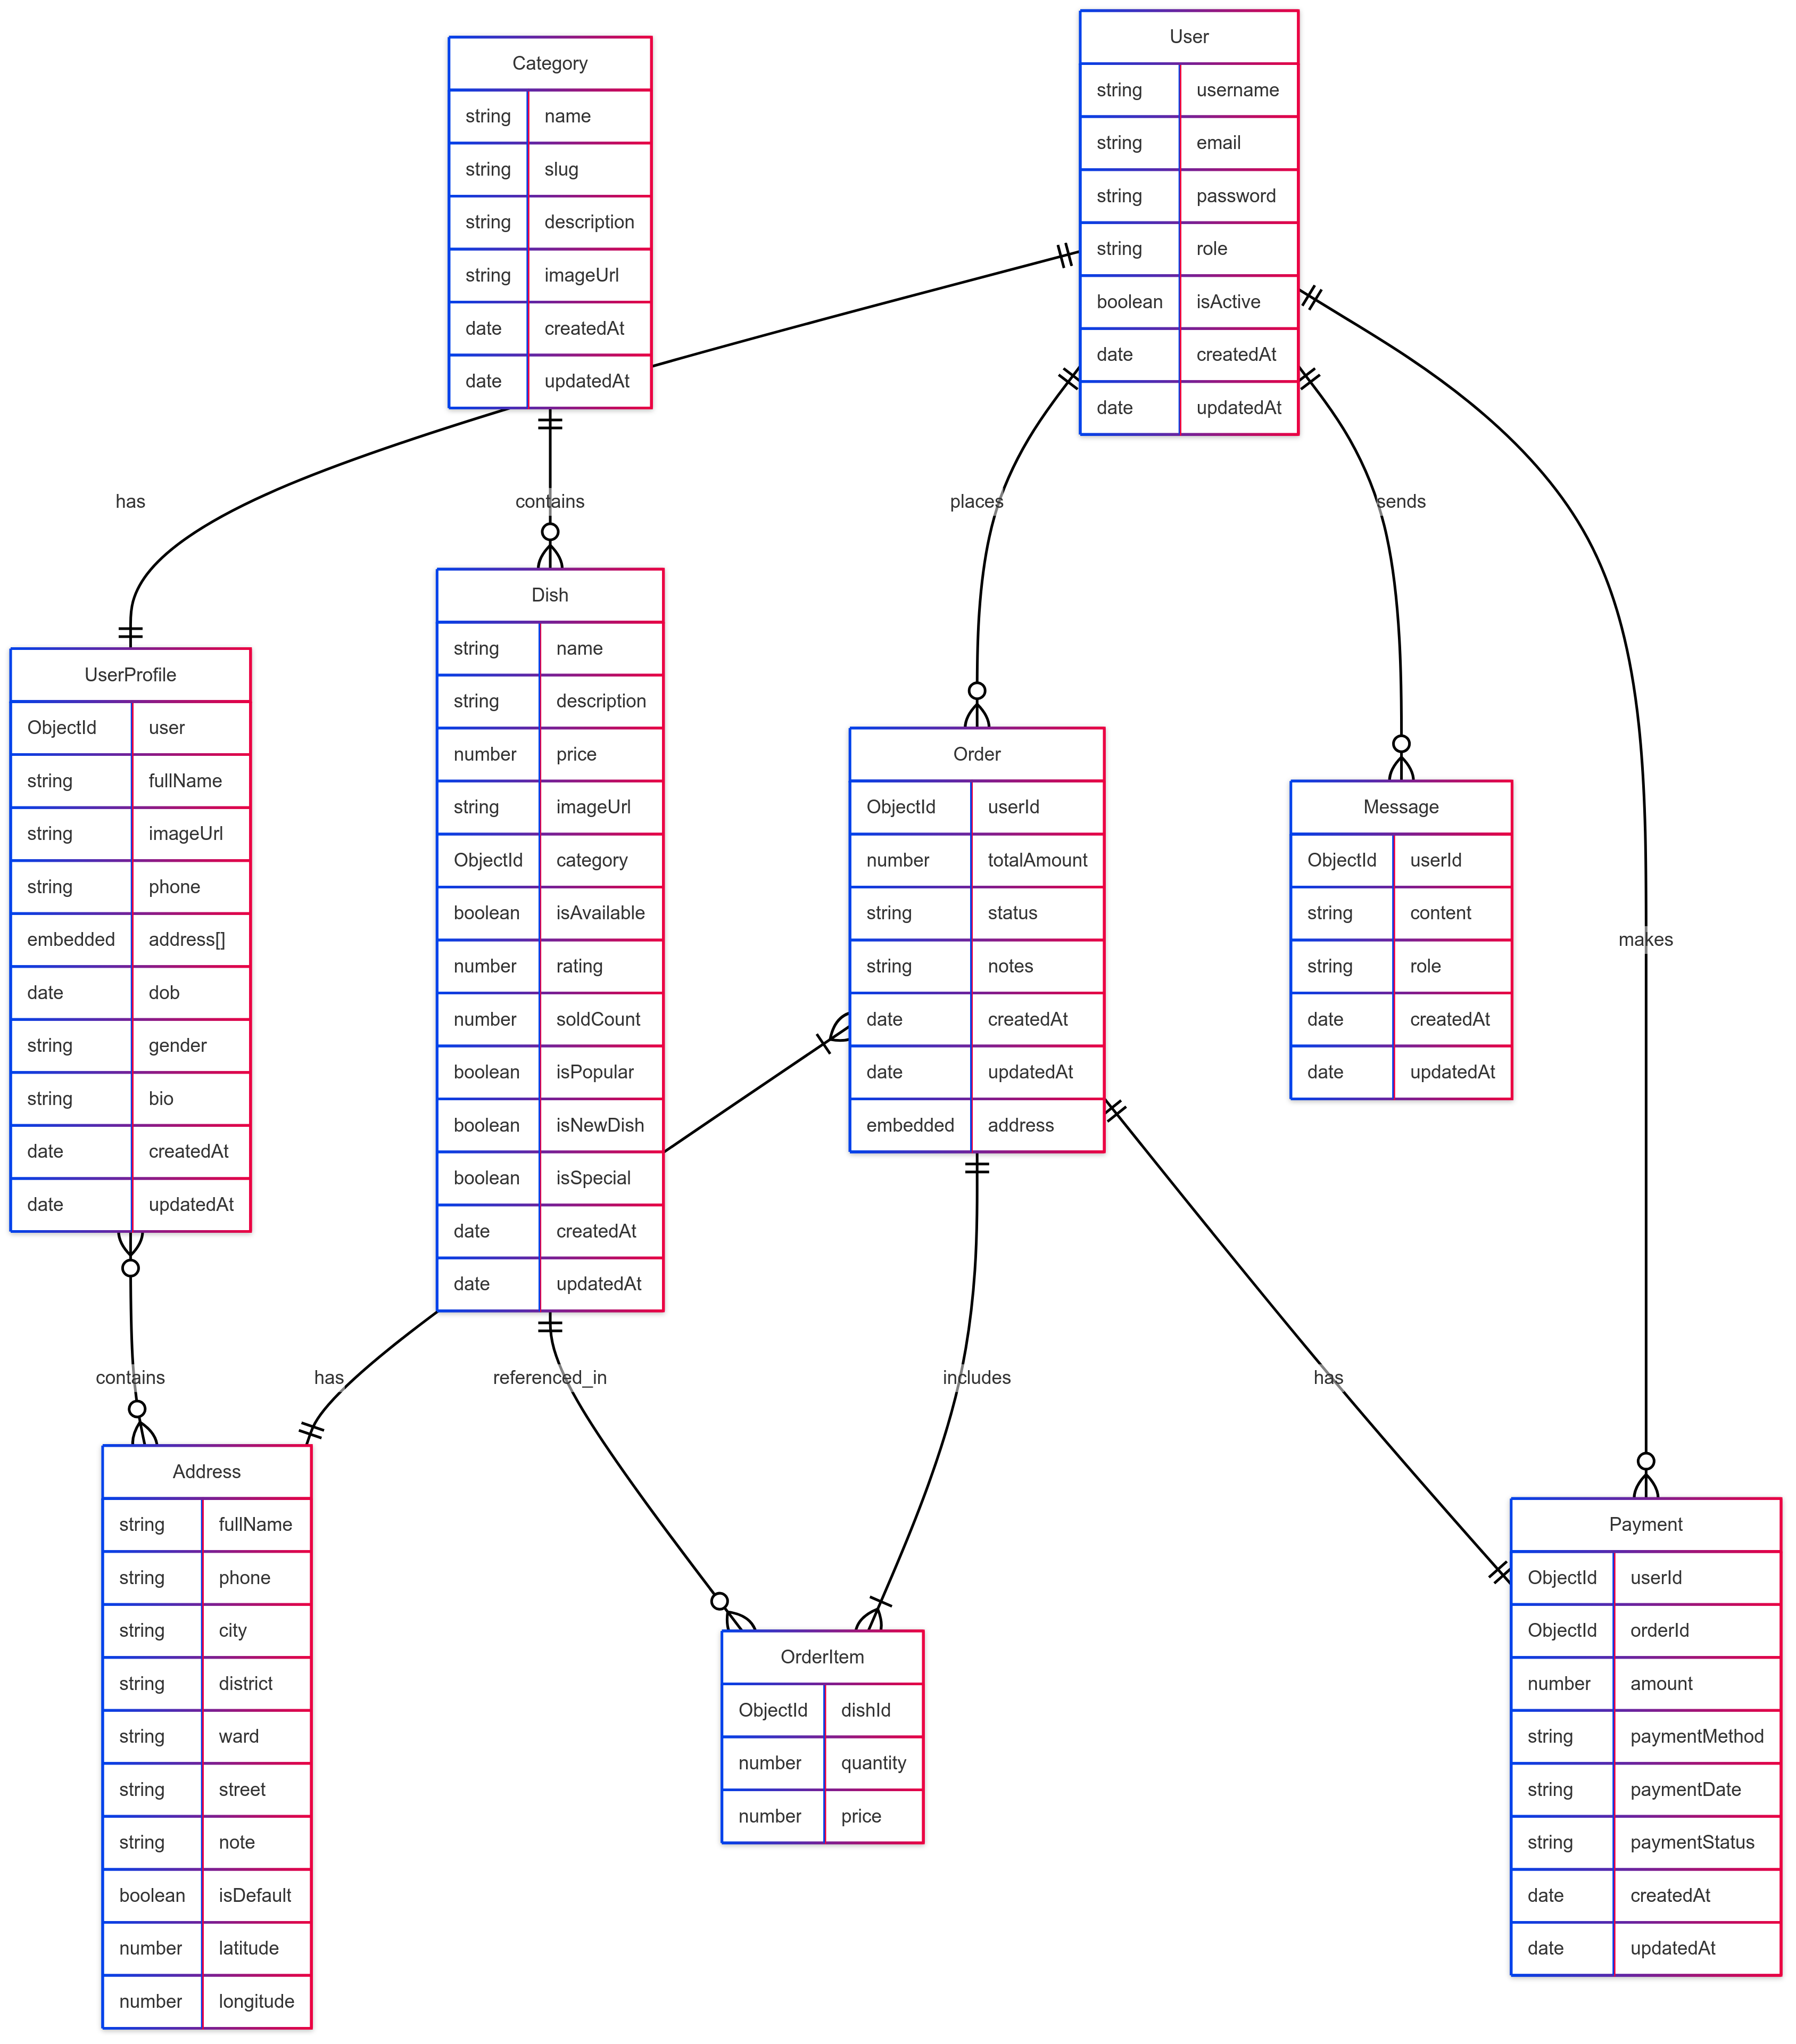
\includegraphics[width=\textwidth]{images/database-diagram.png}
\caption{Sơ đồ cơ sở dữ liệu của hệ thống Việt Food}
\label{fig:database-diagram}
\end{figure}

\subsection{Cơ sở dữ liệu bổ sung}
Bên cạnh MongoDB, hệ thống còn tích hợp:
\begin{itemize}
    \item \textbf{Redis}:
    \begin{itemize}
        \item Caching dữ liệu thường truy cập (thông tin món ăn, danh mục)
        \item Quản lý phiên đăng nhập
        \item Xử lý tin nhắn real-time thông qua Redis Stream
    \end{itemize}
    
    \item \textbf{Elasticsearch}:
    \begin{itemize}
        \item Đánh chỉ mục dữ liệu món ăn
        \item Hỗ trợ tìm kiếm full-text với khả năng ranking
        \item Tìm kiếm gợi ý (suggestions) khi người dùng nhập
    \end{itemize}
\end{itemize}

\subsection{Tối ưu hóa hiệu năng}
\begin{itemize}
    \item \textbf{Indexing}: Các trường thường xuyên truy vấn được đánh index
    \item \textbf{Caching}: Sử dụng Redis để giảm tải cho database chính
    \item \textbf{Phân trang}: Áp dụng cho danh sách món ăn và lịch sử đơn hàng
    \item \textbf{Aggregation}: Tổng hợp dữ liệu thống kê hiệu quả
\end{itemize}

\subsection{Bảo mật dữ liệu}
\begin{itemize}
    \item Mã hóa mật khẩu bằng bcrypt
    \item Xác thực JWT cho API
    \item Phân quyền chi tiết theo vai trò
    \item Kiểm tra quyền truy cập ở tầng middleware
\end{itemize}


\chapter{Phân tích chi tiết các thành phần dự án}
\section{Phân tích chi tiết các thành phần của dự án}

Phần này phân tích chi tiết các thành phần frontend và backend của dự án Việt Food. Chúng tôi sẽ đi sâu vào các tính năng nổi bật, kỹ thuật triển khai, và những giải pháp được áp dụng để đảm bảo hiệu suất và trải nghiệm người dùng tốt.

\section{Frontend - Giao diện người dùng}

\subsection{Cấu trúc component hiện đại}

Frontend của Việt Food được xây dựng bằng React và TypeScript, áp dụng một cấu trúc có tính mô-đun cao và dễ bảo trì. Hệ thống component được tổ chức theo các lớp:

\begin{enumerate}
    \item \textbf{Atomic Design Pattern}: Các component được tổ chức theo mô hình Atoms, Molecules, Organisms, Templates và Pages.
    \item \textbf{Chia nhỏ component}: Các thành phần UI được tách thành các component nhỏ để tăng khả năng tái sử dụng.
    \item \textbf{Cô lập logic}: Logic được tách biệt với giao diện thông qua các custom hooks.
\end{enumerate}

Một ví dụ về cấu trúc component trong Việt Food:

\begin{verbatim}
// Atomic design: Button (Atom)
src/components/ui/button.tsx

// DishCard (Molecule)
src/components/dishes/dish-card.tsx

// DishList (Organism)
src/components/dishes/dish-list.tsx

// HomePage (Page)
src/pages/home.tsx
\end{verbatim}

\subsection{Styling và Thiết kế}

Việt Food sử dụng Tailwind CSS kết hợp với các component từ Radix UI để tạo ra một hệ thống giao diện nhất quán và hiện đại:

\begin{itemize}
    \item \textbf{Utility-first CSS}: Sử dụng các lớp của Tailwind giúp phát triển nhanh và nhất quán.
    \item \textbf{Theme Configuration}: Hệ thống màu sắc, typography, và spacing được cấu hình trong tailwind.config.ts.
    \item \textbf{Component Libraries}: Sử dụng Radix UI làm nền tảng, tùy chỉnh với Tailwind CSS.
    \item \textbf{Responsive Design}: Ứng dụng được thiết kế đáp ứng trên các kích thước màn hình khác nhau.
\end{itemize}

Một ví dụ về cách kết hợp Radix UI và Tailwind CSS:

\begin{verbatim}
// Button component sử dụng Radix UI Slot với Tailwind CSS
import { Slot } from "@radix-ui/react-slot"
import { cva, type VariantProps } from "class-variance-authority"

const buttonVariants = cva(
  "inline-flex items-center justify-center rounded-md text-sm font-medium",
  {
    variants: {
      variant: {
        default: "bg-primary text-primary-foreground hover:bg-primary/90",
        destructive: "bg-destructive text-destructive-foreground hover:bg-destructive/90",
        outline: "border border-input bg-background hover:bg-accent hover:text-accent-foreground",
        // ... các variants khác
      },
      size: {
        default: "h-10 px-4 py-2",
        sm: "h-9 rounded-md px-3",
        lg: "h-11 rounded-md px-8",
      },
    },
    defaultVariants: {
      variant: "default",
      size: "default",
    },
  }
)
\end{verbatim}

\subsection{Quản lý dữ liệu và State Management}

Việt Food sử dụng một hỗn hợp các công cụ để quản lý dữ liệu và trạng thái ứng dụng:

\begin{itemize}
    \item \textbf{React Context API}: Quản lý trạng thái toàn cục của ứng dụng như xác thực người dùng (auth), giỏ hàng (cart).
    \item \textbf{Custom Hooks}: Tạo ra các hooks chuyên biệt như useAuth, useProfile để truy cập và cập nhật trạng thái.
    \item \textbf{Zod}: Validation dữ liệu chặt chẽ với TypeScript.
    \item \textbf{React Hook Form}: Quản lý form với hiệu suất cao.
    \item \textbf{Local Storage}: Lưu trữ access token và refresh token trên client.
\end{itemize}

Ví dụ về việc triển khai Context API và custom hooks để quản lý giỏ hàng:

\begin{verbatim}
// CartContext.tsx
import { createContext, useContext, useState, ReactNode } from "react";

interface CartItem {
  id: string;
  name: string;
  price: number;
  imageUrl: string;
  quantity: number;
}

interface CartContextType {
  cartItems: CartItem[];
  isCartOpen: boolean;
  addToCart: (item: CartItem) => void;
  removeFromCart: (id: string) => void;
  // ... các phương thức khác
}

const CartContext = createContext<CartContextType | undefined>(undefined);

export const CartProvider = ({ children }: { children: ReactNode }) => {
  const [cartItems, setCartItems] = useState<CartItem[]>([]);
  const [isCartOpen, setIsCartOpen] = useState(false);
  
  // Triển khai các phương thức
  
  return (
    <CartContext.Provider value={{ cartItems, isCartOpen, ... }}>
      {children}
    </CartContext.Provider>
  );
};

// Custom hook để sử dụng context
export const useCart = () => {
  const context = useContext(CartContext);
  if (context === undefined) {
    throw new Error("useCart must be used within a CartProvider");
  }
  return context;
};
\end{verbatim}

\begin{verbatim}
function DishListPage() {
  const [filters, setFilters] = useState({
    category: '',
    search: '',
    page: 1
  })
  
  const { data, isLoading, error } = useDishes(filters)
  
  // ...
}
\end{verbatim}

\subsection{Routing và Navigation}

Việt Food sử dụng thư viện wouter cho routing nhẹ nhàng và hiệu quả:

\begin{itemize}
    \item \textbf{Lazy Loading}: Các trang được tải lazy để giảm kích thước bundle ban đầu.
    \item \textbf{Route Protection}: Các route được bảo vệ dựa trên vai trò người dùng.
    \item \textbf{URL Params và Query Strings}: Xử lý các tham số đường dẫn và query string cho tìm kiếm và lọc.
\end{itemize}

Cấu trúc routing trong Việt Food:

\begin{verbatim}
import { Route, Switch } from 'wouter'
import { lazy, Suspense } from 'react'

// Lazy loaded components
const Home = lazy(() => import('./pages/home'))
const DishList = lazy(() => import('./pages/dish-list'))
const DishDetail = lazy(() => import('./pages/dish-detail'))
const Cart = lazy(() => import('./pages/cart'))

function App() {
  return (
    <Suspense fallback={<LoadingSpinner />}>
      <Switch>
        <Route path="/" component={Home} />
        <Route path="/dishes" component={DishList} />
        <Route path="/dishes/:id" component={DishDetail} />
        <Route path="/cart">
          {/* Protected route */}
          {isAuthenticated ? <Cart /> : <Redirect to="/login" />}
        </Route>
        {/* ... more routes */}
      </Switch>
    </Suspense>
  )
}
\end{verbatim}

\subsection{Optimization tại Frontend}

Frontend của Việt Food áp dụng nhiều kỹ thuật tối ưu hoá để đảm bảo hiệu suất cao:

\begin{itemize}
    \item \textbf{Code Splitting}: Chia nhỏ bundle JS thông qua lazy loading.
    \item \textbf{Memoization}: Sử dụng React.memo, useMemo, và useCallback để giảm re-renders không cần thiết.
    \item \textbf{Virtualization}: Sử dụng windowing cho danh sách dài.
    \item \textbf{Image Optimization}: Sử dụng các kỹ thuật lazy loading, responsive images, và next-gen formats (WebP).
    \item \textbf{Bundle Optimization}: Sử dụng Vite để bundling nhanh và hiệu quả.
\end{itemize}

Ví dụ về tối ưu hoá component với memoization:

\begin{verbatim}
import { memo, useMemo, useCallback } from 'react'

// Memoized component để tránh re-renders không cần thiết
const DishCard = memo(function DishCard({ dish, onAddToCart }) {
  // Xử lý component rendering
  return (
    <div className="dish-card">
      <img 
        src={dish.imageUrl} 
        alt={dish.name}
        loading="lazy" // Lazy load images
      />
      <h3>{dish.name}</h3>
      <p>{dish.price.toLocaleString('vi-VN')} đ</p>
      <button onClick={() => onAddToCart(dish)}>Thêm vào giỏ</button>
    </div>
  )
})

function DishList({ dishes }) {
  // Memoize expensive calculations
  const sortedDishes = useMemo(() => {
    return [...dishes].sort((a, b) => a.price - b.price)
  }, [dishes])
  
  // Memoize callback functions
  const handleAddToCart = useCallback((dish) => {
    // Logic để thêm vào giỏ hàng
  }, [])
  
  return (
    <div className="dish-grid">
      {sortedDishes.map(dish => (
        <DishCard 
          key={dish.id} 
          dish={dish} 
          onAddToCart={handleAddToCart}
        />
      ))}
    </div>
  )
}
\end{verbatim}

\section{Backend - Kỹ thuật tối ưu hóa}

\subsection{Redis Caching}

\subsection{Khái niệm và lợi ích}
Redis là hệ thống lưu trữ dữ liệu key-value trong bộ nhớ, có khả năng lưu trữ nhiều kiểu dữ liệu khác nhau. Trong Việt Food, Redis được sử dụng chủ yếu làm hệ thống cache để tối ưu hóa thời gian truy vấn dữ liệu:

\begin{itemize}
    \item \textbf{Tốc độ truy xuất nhanh}: Dữ liệu được lưu trong bộ nhớ, giảm độ trễ so với truy vấn database
    \item \textbf{Giảm tải cho database chính}: Các truy vấn phổ biến được cache, giảm số lượng truy cập vào MongoDB
    \item \textbf{Tăng khả năng phục vụ đồng thời}: Hệ thống có thể xử lý nhiều request hơn trong cùng một thời điểm
\end{itemize}

\subsection{Triển khai trong dự án}
Trong Việt Food, Redis được cấu hình và khởi tạo trong file \texttt{config/redis.ts}:

\begin{verbatim}
import Redis from "ioredis"
import { REDIS_PORT, REDIS_HOST } from "../config"

const redis = new Redis({
    host: REDIS_HOST,
    port: REDIS_PORT,
})

redis.on("connect", () => {
    console.log(`[SUCCESS] Redis connected: ${redis.options.host}:${redis.options.port}`)
})

redis.on("error", (err) => {
    console.error(err)
})

export default redis
\end{verbatim}

\subsection{Cache dữ liệu món ăn}
Dữ liệu món ăn là loại dữ liệu được truy cập thường xuyên nhưng ít thay đổi, nên việc cache là rất hiệu quả. Trong \texttt{DishService}, các phương thức tìm kiếm món ăn đều áp dụng caching:

\begin{verbatim}
// Lấy món ăn theo ID với cache
static async findById(id: string | Types.ObjectId): Promise<IDishDocument | null> {
    const cacheKey = `dish:${id}`
    const cachedDish = await redis.get(cacheKey)
    
    if (cachedDish) {
        return JSON.parse(cachedDish)
    }
    
    const dish = await DishModel.findById(id).populate('category').lean()
    if (dish) {
        await redis.set(cacheKey, JSON.stringify(dish), 'EX', 3600 * 24)
        return dish
    }
    
    return null
}
\end{verbatim}

\subsection{Prime Cache khi khởi động}
Một điểm đáng chú ý là Việt Food sử dụng kỹ thuật "prime cache" khi khởi động server - tức là nạp trước dữ liệu phổ biến vào cache:

\begin{verbatim}
static async primeAllDishesCache(): Promise<void> {
    try {
        const allDishes = await DishModel.find({ isAvailable: true }).lean()
        if (allDishes && allDishes.length > 0) {
            const pipeline = redis.pipeline()
            for (const dish of allDishes) {
                const cacheKey = `dish:${dish._id}`
                dish.imageUrl = getFullImageUrl(dish.imageUrl)
                pipeline.set(cacheKey, JSON.stringify(dish), 'EX', 3600 * 24)
            }
            await pipeline.exec()
        }
    } catch (error) {
        console.error('Error priming all dishes cache:', error)
    }
}
\end{verbatim}

Phương thức này được gọi khi server khởi động trong \texttt{server.ts}:

\begin{verbatim}
connectDB();
connectElasticsearch();
DishService.primeAllDishesCache()
\end{verbatim}

\subsection{Invalidation cache}
Khi dữ liệu thay đổi, cache cần được cập nhật hoặc xóa để tránh dữ liệu không đồng bộ. Việt Food xử lý vấn đề này bằng cách xóa các key cache liên quan khi có thay đổi:

\begin{verbatim}
// Xóa cache khi cập nhật món ăn
const keys = await redis.keys('dishes:*')
if (keys.length > 0) {
    const pipeline = redis.pipeline()
    keys.forEach(key => pipeline.del(key))
    await pipeline.exec()
}
\end{verbatim}

\section{Redis Stream}

\subsection{Khái niệm và lợi ích}
Redis Stream là một cấu trúc dữ liệu mới trong Redis, cho phép lưu trữ và quản lý các dòng sự kiện theo thời gian thực, tương tự như một message broker:

\begin{itemize}
    \item \textbf{Xử lý tin nhắn không đồng bộ}: Các thành phần khác nhau có thể giao tiếp mà không cần chờ đợi nhau
    \item \textbf{Mô hình publish-subscribe}: Phân tách giữa producer và consumer
    \item \textbf{Khả năng mở rộng}: Nhiều consumer có thể xử lý cùng một stream
    \item \textbf{Độ tin cậy}: Tin nhắn được lưu trữ lâu dài và có thể được xử lý lại nếu cần
\end{itemize}

\subsection{Triển khai trong dự án}
Trong Việt Food, Redis Stream được sử dụng chủ yếu để xử lý tin nhắn. Đầu tiên, stream key được định nghĩa trong file cấu hình Redis:

\begin{verbatim}
export const MESSAGE_STREAM_KEY = "message_stream";
\end{verbatim}

MessageWorkerService xử lý tin nhắn từ stream:

\begin{verbatim}
export default class MessageWorkerService {
    static async createConsumerGroup() {
        try {
            const streamExists = await redis.exists(MESSAGE_STREAM_KEY);
            if (!streamExists) {
                await redis.xgroup('CREATE', MESSAGE_STREAM_KEY, GROUP_NAME, '0', 'MKSTREAM');
            }
        } catch (error) {
            console.log('error', error);
        }
    }

    static async processStreamMessages() {
        while (true) {
            try {
                const result = await redis.xreadgroup(
                    'GROUP', GROUP_NAME,
                    CONSUMER_NAME,
                    'COUNT', 1,
                    'BLOCK', 0,
                    'STREAMS', MESSAGE_STREAM_KEY,
                    '>'
                ) as XReadGroupResult;

                const message = this.convertStreamMessageToObject(result?.[0]?.[1]?.[0]?.[1]);
                if (message) {
                    await MessageService.createMessage(message.userId, message.content, message.role);
                }
            } catch (error) {
                console.error('Error processing stream messages:', error);
            }
        }
    }
}
\end{verbatim}

Stream consumer được khởi động riêng biệt từ file \texttt{consumer.ts}:

\begin{verbatim}
import MessageWorkerService from './services/message-worker.service';

(async () => {
    await MessageWorkerService.createConsumerGroup();
    await MessageWorkerService.processStreamMessages();
})();
\end{verbatim}

\section{HTTP Compression}

\subsection{Khái niệm và lợi ích}
HTTP Compression là kỹ thuật nén dữ liệu trước khi gửi từ server đến client, giúp giảm kích thước dữ liệu truyền tải:

\begin{itemize}
    \item \textbf{Giảm băng thông}: Tiết kiệm băng thông và chi phí mạng
    \item \textbf{Tăng tốc độ tải trang}: Người dùng nhận được phản hồi nhanh hơn
    \item \textbf{Cải thiện trải nghiệm}: Đặc biệt hiệu quả với người dùng có kết nối mạng chậm
\end{itemize}

\subsection{Triển khai trong dự án}
Việt Food sử dụng middleware \texttt{compression} của Express để nén dữ liệu:

\begin{verbatim}
import compression from "compression";

const compressOptions = {
    threshold: 1024,  // Chỉ nén dữ liệu lớn hơn 1KB
    level: 6,        // Mức độ nén từ 1-9, cân bằng giữa tốc độ và hiệu quả nén
}

app.use(compression(compressOptions));
\end{verbatim}

Cấu hình này được thiết lập trong \texttt{server.ts}, áp dụng cho tất cả các request. Điểm đáng chú ý:

\begin{itemize}
    \item \textbf{threshold 1024 bytes}: Chỉ nén các phản hồi có kích thước lớn hơn 1KB, tránh lãng phí tài nguyên CPU cho các phản hồi nhỏ
    \item \textbf{level 6}: Mức nén cân bằng giữa tốc độ và hiệu quả nén
\end{itemize}

\section{Tối ưu hóa hình ảnh với Sharp}

\subsection{Khái niệm và lợi ích}
Sharp là thư viện xử lý hình ảnh cho Node.js, được xây dựng trên libvips - thư viện xử lý hình ảnh hiệu suất cao:

\begin{itemize}
    \item \textbf{Tốc độ xử lý cao}: Nhanh hơn nhiều so với các thư viện xử lý ảnh thông thường
    \item \textbf{Tiết kiệm bộ nhớ}: Sử dụng bộ nhớ hiệu quả khi xử lý ảnh lớn
    \item \textbf{Tối ưu hóa định dạng}: Chuyển đổi sang các định dạng hiệu quả như WebP
    \item \textbf{Thay đổi kích thước}: Giảm kích thước ảnh nhưng vẫn giữ chất lượng tốt
\end{itemize}

\subsection{Triển khai trong dự án}
Việt Food sử dụng Sharp thông qua middleware \texttt{image-processor.middleware.ts} để xử lý ảnh khi người dùng tải lên:

\begin{verbatim}
import sharp from 'sharp';
import fs from 'fs';
import path from 'path';

const processOneImage = async (file: Express.Multer.File): Promise<void> => {
    const originalPath = file.path;
    const fileDir = path.dirname(originalPath);
    const filename = path.basename(originalPath, path.extname(originalPath));
    const webpFilename = `${filename}.webp`;
    const outputPath = path.join(fileDir, webpFilename);

    await sharp(originalPath)
        .resize(1000)
        .webp({
            quality: 80,
            effort: 6  
        })
        .toFile(outputPath);

    fs.unlinkSync(originalPath);

    file.path = outputPath;
    file.filename = webpFilename;
    file.mimetype = 'image/webp';
};
\end{verbatim}

Middleware này thực hiện các tối ưu:

\begin{itemize}
    \item \textbf{Resize}: Giảm kích thước ảnh xuống tối đa 1000px để tiết kiệm không gian lưu trữ
    \item \textbf{Chuyển đổi sang WebP}: Định dạng hiện đại có kích thước nhỏ hơn nhưng chất lượng tương đương hoặc tốt hơn JPEG/PNG
    \item \textbf{Điều chỉnh chất lượng}: Cân bằng giữa kích thước file và chất lượng hình ảnh (quality: 80)
    \item \textbf{Mức độ nén tối ưu}: Cấu hình effort: 6 đảm bảo cân bằng giữa tốc độ xử lý và hiệu quả nén
\end{itemize}

Middleware này được áp dụng cho các route xử lý upload hình ảnh, đảm bảo tất cả hình ảnh đều được tối ưu trước khi lưu trữ.

\section{Tích hợp và tương tác giữa các kỹ thuật}

Các kỹ thuật tối ưu trong Việt Food không hoạt động độc lập mà bổ trợ cho nhau:

\begin{itemize}
    \item \textbf{Sharp + Redis}: Hình ảnh được tối ưu với Sharp, sau đó URL được lưu trong Redis cache
    \item \textbf{Redis Cache + Compression}: Dữ liệu được cache và nén khi truyền tải, giảm thời gian tải trang
    \item \textbf{Redis Stream + Services}: Xử lý tin nhắn không đồng bộ, giải phóng server chính để xử lý các request khác
\end{itemize}

Việc kết hợp các kỹ thuật này tạo nên một pipeline tối ưu, từ khi dữ liệu được tạo ra, lưu trữ đến khi được truyền tải đến người dùng cuối.

\section{Hệ thống Agent thông minh}

\subsection{Giới thiệu về Agent}

Việt Food triển khai một hệ thống Agent thông minh hỗ trợ khách hàng trong quá trình đặt món và tương tác với ứng dụng:

\begin{itemize}
    \item \textbf{Trợ lý ảo}: Agent hoạt động như một trợ lý ảo thông minh, tương tác với người dùng qua giao diện chat
    \item \textbf{Xử lý ngôn ngữ tự nhiên}: Sử dụng mô hình NLP để hiểu và phản hồi câu hỏi của người dùng
    \item \textbf{Tư vấn món ăn}: Gợi ý món ăn dựa trên sở thích và lịch sử đặt hàng của người dùng
    \item \textbf{Xử lý quy trình}: Hướng dẫn người dùng hoàn thành quy trình đặt hàng
\end{itemize}

\subsection{Kiến trúc Agent}

Hệ thống Agent được xây dựng với kiến trúc microservice, tách biệt với core service chính:

\begin{verbatim}
// agent-service.ts
export class AgentService {
    private nlpProcessor: NLPProcessor;
    private recommendationEngine: RecommendationEngine;
    
    constructor() {
        this.nlpProcessor = new NLPProcessor();
        this.recommendationEngine = new RecommendationEngine();
    }
    
    async processUserMessage(userId: string, message: string): Promise<AgentResponse> {
        // Xử lý tin nhắn từ người dùng
        const intent = await this.nlpProcessor.detectIntent(message);
        
        // Lưu tin nhắn vào cơ sở dữ liệu
        await this.storeMessage(userId, message, 'user');
        
        // Tạo phản hồi dựa trên intent
        const response = await this.generateResponse(userId, intent, message);
        
        // Lưu phản hồi của Agent
        await this.storeMessage(userId, response.content, 'agent');
        
        return response;
    }
    
    private async generateResponse(userId: string, intent: Intent, message: string): Promise<AgentResponse> {
        switch (intent.type) {
            case 'DISH_RECOMMENDATION':
                return await this.recommendationEngine.getRecommendations(userId, intent.parameters);
            case 'ORDER_STATUS':
                return await this.getOrderStatus(userId);
            // Xử lý các intent khác
            default:
                return { content: 'Xin lỗi, tôi không hiểu yêu cầu của bạn.' };
        }
    }
}
\end{verbatim}

\subsection{Lưu trữ message và quản lý context}

Một trong những thách thức lớn nhất của hệ thống Agent là việc lưu trữ tin nhắn và duy trì context hội thoại. Việt Food sử dụng MongoDB để lưu trữ tin nhắn và Redis để quản lý context session:

\begin{verbatim}
// message.model.ts
import { Schema, model, Types, Document } from "mongoose";

export enum MessageRole {
    USER = "user",
    ASSISTANT = "assistant",
}

export interface IMessage {
    userId: Types.ObjectId;
    content: string;
    role: MessageRole;
}

const messageSchema = new Schema({
    userId: { type: Schema.Types.ObjectId, ref: "User", required: true },
    content: { type: String, required: true },
    role: { type: String, enum: MessageRole, required: true },
}, { timestamps: true });

const Message = model("Message", messageSchema);
\end{verbatim}

Dịch vụ MessageService cung cấp các phương thức để lưu trữ và truy xuất tin nhắn, kết hợp với Redis Stream để xử lý bất đồng bộ:

\begin{verbatim}
// message.service.ts
import redis from "@/config/redis";
import Message, { MessageRole } from "@/model/message.model";
import { Types } from "mongoose";

export const MESSAGE_STREAM_KEY = "message_stream";
export const MESSAGE_GROUP_NAME = "message_group";

export default class MessageService {
    static async createMessage(userId: Types.ObjectId, content: string, role: MessageRole) {
        const newMessage = await Message.create({ userId, content, role });
        return newMessage;
    }

    static async getMessagesByUserId(userId: Types.ObjectId) {
        const messages = await Message.find({ userId }).sort({ createdAt: -1 }).lean();
        return messages;
    }

    static addMessageToStream = async (streamKey: string, message: Record<string, any>): Promise<string | null> => {
        const result = await redis.xadd(streamKey, "*", ...Object.entries(message).flat());
        return result;
    }
}
\end{verbatim}

\subsection{Quản lý context hội thoại}

Duy trì context hội thoại là yếu tố quan trọng để Agent có thể hiểu được tiến trình đối thoại đang diễn ra. Trong hệ thống Việt Food, context hội thoại được xây dựng bằng cách kết hợp lịch sử tin nhắn với trạng thái hội thoại hiện tại. Mỗi trạng thái hội thoại có thể bao gồm các thông tin quan trọng như:

\begin{itemize}
    \item \textbf{Trạng thái hội thoại}: Đang tìm kiếm món ăn, đang xác nhận đơn hàng, v.v.
    \item \textbf{Thông tin người dùng}: Sở thích, ràng buộc ăn uống, địa chỉ giao hàng
    \item \textbf{Giỏ hàng hiện tại}: Các món ăn đã được thêm vào giỏ hàng trong cuộc hội thoại
    \item \textbf{Intent trước đó}: Mục đích giao tiếp trước đó của người dùng
\end{itemize}

Một phương pháp tối ưu để quản lý context hội thoại có thể được triển khai bằng cách sử dụng Google GenAI và in-memory cache, với định nghĩa cơ bản như sau:

\begin{verbatim}
// agent.service.ts
import { Chat, FunctionCall, GoogleGenAI } from "@google/genai";
import { GEMINI_API_KEY, MODEL } from "@/config";

interface AgentSessionEntry {
    chat: Chat;
    lastAccessed: number;
}

export class Agent {
    static gemini = new GoogleGenAI({
        apiKey: GEMINI_API_KEY,
    });

    static agentSessionMap = new Map<string, AgentSessionEntry>();

    static readonly SESSION_TTL = 1 * 60 * 60 * 1000; // 1 giờ

    static getOrCreateAgentSession = (user: IUserDocument): Chat => {
        const userId = user?.id;
        let sessionEntry = this.agentSessionMap.get(userId);

        if (sessionEntry) {
            const currentTime = Date.now();
            if (currentTime - sessionEntry.lastAccessed > this.SESSION_TTL) {
                this.agentSessionMap.delete(userId);
                sessionEntry = undefined;
            } else {
                sessionEntry.lastAccessed = currentTime;
                return sessionEntry.chat;
            }
        }

        const newAgentSession: Chat = this.gemini.chats.create({
            model: MODEL,
            config: {
                tools,
                responseMimeType: 'text/plain',
                systemInstruction: `Bạn là nhân viên bán món ăn của cửa hàng Việt Food đang trò chuyện với ${user?.username}. Hãy trả lời vui vẻ, thân thiện, kèm theo các emoji. Hãy nói chuyện sao cho khách hàng đủ mua món ăn.`,
                maxOutputTokens: 500,
                topP: 0
            }
        });

        this.agentSessionMap.set(userId, {
            chat: newAgentSession,
            lastAccessed: Date.now()
        });

        return newAgentSession;
    }
}
\end{verbatim}

Phương pháp này mang lại nhiều ưu điểm quan trọng:

\begin{itemize}
    \item \textbf{Context tự động}: Google Gemini tự động duy trì context hội thoại, giảm thiểu việc sử dụng
    \item \textbf{In-memory cache}: Các phiên hội thoại (Chat Session) được lưu trữ trong Map với thời gian sống là 1 giờ
    \item \textbf{Tích hợp tools}: Hệ thống sử dụng các function tools (Function Calling) để Agent có thể thực hiện các tác vụ như tìm kiếm món ăn, thêm vào giỏ hàng
\end{itemize}

Các function tool quan trọng được triển khai cho hệ thống bao gồm:

\begin{itemize}
    \item \textbf{searchDishes}: Tìm kiếm món ăn theo các tiêu chí
    \item \textbf{addToCart}: Thêm món ăn vào giỏ hàng
    \item \textbf{removeFromCart}: Xóa món ăn khỏi giỏ hàng
    \item \textbf{getDishesInUserCart}: Lấy danh sách món ăn trong giỏ hàng
    \item \textbf{getAllDishes}: Lấy toàn bộ danh sách món ăn
\end{itemize}

Việc kết hợp Google GenAI, in-memory cache, và các function tool tạo nên một hệ thống Agent thông minh có khả năng duy trì cuộc hội thoại mạch lạc với người dùng. Context được duy trì xuyên suốt cuộc hội thoại giúp Agent hiểu được ý định và mong muốn của người dùng, đồng thời thực hiện các tác vụ cần thiết như tìm kiếm món ăn và đặt hàng.


\chapter{Đánh giá hiệu quả và đề xuất cải tiến}
\section{Đánh giá tổng thể dự án}

Sau khi phân tích chi tiết các thành phần của dự án Việt Food, phần này đánh giá hiệu quả tổng thể của dự án, xem xét cả frontend và backend, đồng thời chỉ ra ưu điểm và hạn chế của cách triển khai hiện tại.

\section{Ưu điểm của mã nguồn}

\subsection{Frontend}
\begin{itemize}
    \item \textbf{Kiến trúc component mạch lạc}: Sử dụng Atomic Design Pattern giúp code dễ bảo trì, mở rộng và tái sử dụng.
    \item \textbf{Tách biệt logic và UI}: Sử dụng custom hooks để tách biệt logic nghiệp vụ khỏi giao diện.
    \item \textbf{React Query}: Sử dụng hiệu quả để quản lý dữ liệu server-side, bao gồm cache và invalidation.
    \item \textbf{Tối ưu hóa hiệu suất}: Áp dụng các kỹ thuật như code splitting, lazy loading, và memoization.
    \item \textbf{Sử dụng Tailwind và Radix UI}: Kết hợp hiệu quả giữa utility-first CSS và headless UI components.
    \item \textbf{Responsive design}: Giao diện đáp ứng tốt trên các kích thước màn hình khác nhau.
    \item \textbf{Strong typing}: Sử dụng TypeScript và Zod giúp phát hiện lỗi sớm và đảm bảo type safety.
\end{itemize}

\subsection{Redis Caching}
\begin{itemize}
    \item \textbf{Áp dụng hợp lý}: Cache được áp dụng cho các dữ liệu thường xuyên được truy cập nhưng ít thay đổi như thông tin món ăn và danh mục.
    \item \textbf{Chiến lược priming thông minh}: Việc nạp trước dữ liệu phổ biến vào cache khi khởi động server giúp tăng hiệu suất ngay từ đầu.
    \item \textbf{Thời gian hết hạn phù hợp}: Các key cache có thời gian hết hạn khác nhau tùy theo loại dữ liệu, ví dụ:
    \begin{verbatim}
    // Dữ liệu chi tiết món ăn - 24 giờ
    await redis.set(cacheKey, JSON.stringify(dish), 'EX', 3600 * 24)
    
    // Danh sách món ăn theo query - 10 phút
    await redis.set(cacheKey, JSON.stringify(result), 'EX', 600)
    
    // Món ăn phổ biến - 6 giờ
    await redis.set(cacheKey, JSON.stringify(popularDishes), 'EX', 3600 * 6)
    \end{verbatim}
    \item \textbf{Sử dụng pipeline}: Việc sử dụng Redis pipeline khi thực hiện nhiều thao tác liên tiếp giúp giảm độ trễ mạng, tăng hiệu suất.
\end{itemize}

\subsection{Redis Stream}
\begin{itemize}
    \item \textbf{Kiến trúc phân tách}: Tách biệt xử lý tin nhắn khỏi luồng chính của ứng dụng, giúp giảm tải cho server chính.
    \item \textbf{Khả năng phục hồi}: Cơ chế consumer group đảm bảo tin nhắn vẫn được xử lý ngay cả khi có lỗi.
    \item \textbf{Mở rộng dễ dàng}: Có thể thêm nhiều consumer để xử lý song song nếu cần.
\end{itemize}

\subsection{HTTP Compression}
\begin{itemize}
    \item \textbf{Cấu hình cân bằng}: Cấu hình compression với ngưỡng 1KB và mức nén 6 là cân bằng hợp lý giữa hiệu quả nén và tài nguyên CPU.
    \item \textbf{Áp dụng toàn cục}: Compression được áp dụng như middleware cho tất cả các response, đảm bảo tính nhất quán.
\end{itemize}

\subsection{Tối ưu hình ảnh với Sharp}
\begin{itemize}
    \item \textbf{Chuyển đổi định dạng thông minh}: Chuyển đổi sang WebP giúp giảm đáng kể kích thước file (trung bình 30-50\% so với JPEG và 80\% so với PNG) mà vẫn duy trì chất lượng.
    \item \textbf{Resize tự động}: Giới hạn kích thước hình ảnh ở mức 1000px là đủ cho hầu hết trường hợp sử dụng trên web.
    \item \textbf{Triển khai dưới dạng middleware}: Cách triển khai này đảm bảo tất cả hình ảnh tải lên đều được xử lý đồng nhất.
\end{itemize}

\section{Nhược điểm và hạn chế}

\subsection{Frontend}
\begin{itemize}
    \item \textbf{Chưa có SSR/SSG}: Hiện tại Việt Food sử dụng Client-Side Rendering (CSR) với Vite, chưa áp dụng Server-Side Rendering hoặc Static Site Generation, ảnh hưởng đến SEO và thời gian tải trang ban đầu.
    \item \textbf{Bundle size lớn}: Mặc dù đã có code-splitting, nhưng có nhiều thư viện lớn từ Radix UI, Chart.js, và Framer Motion làm tăng kích thước bundle.
    \item \textbf{Quá phụ thuộc vào React Query}: Sử dụng React Query trong hầu hết các component làm tăng sự phụ thuộc vào một thư viện bên ngoài.
    \item \textbf{Chưa có test coverage đầy đủ}: Thiếu các unit test và integration test cho các component và custom hooks.
    \item \textbf{Tài nguyên hình ảnh chưa được tối ưu hoá đầy đủ}: Chưa có cơ chế lazy loading hình ảnh tự động và next-gen format (WebP, AVIF) ở phía client.
\end{itemize}

\subsection{Redis Caching}
\begin{itemize}
    \item \textbf{Chiến lược invalidation chưa tinh tế}: Hiện tại, khi có cập nhật, dự án xóa tất cả các key cache liên quan đến danh sách món ăn. Cách tiếp cận này đơn giản nhưng có thể gây lãng phí khi một số cache vẫn có thể tái sử dụng.
    \begin{verbatim}
    // Xóa tất cả cache liên quan đến danh sách món ăn
    const keys = await redis.keys('dishes:*')
    if (keys.length > 0) {
        const pipeline = redis.pipeline()
        keys.forEach(key => pipeline.del(key))
        await pipeline.exec()
    }
    \end{verbatim}
    \item \textbf{Thiếu cơ chế phát hiện lỗi cache}: Chưa có cơ chế fallback hoặc circuit breaker nếu Redis gặp sự cố.
    \item \textbf{Chưa tận dụng tối đa tính năng của Redis}: Dự án chưa sử dụng các cấu trúc dữ liệu phức tạp của Redis như sorted sets, lists để tối ưu hơn nữa.
\end{itemize}

\subsection{Redis Stream}
\begin{itemize}
    \item \textbf{Xử lý lỗi còn đơn giản}: Khi gặp lỗi xử lý tin nhắn, hệ thống chỉ ghi log lỗi mà không có cơ chế retry phức tạp hoặc dead letter queue.
    \item \textbf{Thiếu cơ chế giám sát}: Chưa có metrics hoặc monitoring cho việc xử lý stream.
\end{itemize}

\subsection{HTTP Compression}
\begin{itemize}
    \item \textbf{Áp dụng đơn điệu}: Compression được áp dụng đồng đều cho tất cả các route mà không phân biệt loại dữ liệu.
    \item \textbf{Thiếu header điều khiển cache}: Chưa kết hợp tốt giữa compression và HTTP caching headers.
\end{itemize}

\subsection{Tối ưu hình ảnh với Sharp}
\begin{itemize}
    \item \textbf{Kích thước cố định}: Resize cố định ở mức 1000px có thể không phù hợp cho tất cả trường hợp sử dụng.
    \item \textbf{Thiếu responsive images}: Chưa tạo nhiều phiên bản hình ảnh với kích thước khác nhau cho các thiết bị khác nhau.
\end{itemize}

\section{Đề xuất cải tiến}

\subsection{Frontend}
\begin{itemize}
    \item \textbf{Áp dụng Next.js hoặc Astro}: Chuyển sang các framework hỗ trợ SSR/SSG để cải thiện SEO và thời gian tải trang ban đầu.
    \item \textbf{Tree-shaking các thư viện}: Tối ưu hóa bundle size bằng cách import có chọn lọc các component từ Radix UI và các thư viện khác.
    \item \textbf{Tách biệt logic data-fetching}: Giảm sự phụ thuộc vào React Query bằng cách tạo lớp trung gian giữa API calls và React Query.
    \item \textbf{Tăng test coverage}: Thêm unit tests và integration tests cho các component và hooks chính sử dụng Jest và React Testing Library.
    \item \textbf{Tối ưu hóa hình ảnh}: Sử dụng next-gen formats (WebP/AVIF), responsive images và image CDN.
    \item \textbf{Web Vitals monitoring}: Thiết lập hệ thống theo dõi các Core Web Vitals để đánh giá hiệu suất thực tế.
    \item \textbf{Client-side caching}: Triển khai Service Worker và PWA để cải thiện trải nghiệm offline và giảm tải cho server.
\end{itemize}

\subsection{Redis Caching}
\begin{itemize}
    \item \textbf{Invalidation có chọn lọc}: Thay vì xóa tất cả cache, có thể áp dụng cơ chế cache tagging để chỉ xóa những cache bị ảnh hưởng bởi thay đổi.
    \item \textbf{Cơ chế fallback}: Thêm try-catch và circuit breaker pattern khi tương tác với Redis.
    \item \textbf{Tận dụng Redis Pub/Sub}: Kết hợp với Redis Pub/Sub để thông báo invalidation cache giữa nhiều instance của ứng dụng.
    \item \textbf{Áp dụng caching ở nhiều lớp}: Kết hợp với HTTP caching để tối ưu hơn nữa.
\end{itemize}

\subsection{Redis Stream}
\begin{itemize}
    \item \textbf{Consumer groups nâng cao}: Thêm nhiều consumer trong cùng một group để xử lý song song.
    \item \textbf{Cơ chế retry có kiểm soát}: Thêm logic để thử lại xử lý tin nhắn với giới hạn số lần và khoảng thời gian tăng dần.
    \item \textbf{Dead letter queue}: Chuyển tin nhắn không thể xử lý sau nhiều lần thử vào một stream riêng để kiểm tra sau.
\end{itemize}

\subsection{HTTP Compression}
\begin{itemize}
    \item \textbf{Brotli compression}: Xem xét sử dụng Brotli thay vì gzip cho hiệu suất nén tốt hơn trên các trình duyệt hiện đại.
    \item \textbf{Compression có điều kiện}: Áp dụng các mức nén khác nhau cho các loại dữ liệu và endpoint khác nhau.
    \item \textbf{Pre-compressed assets}: Tạo sẵn phiên bản nén của các tài nguyên tĩnh.
\end{itemize}

\subsection{Tối ưu hình ảnh với Sharp}
\begin{itemize}
    \item \textbf{Tạo nhiều kích thước}: Tạo và lưu trữ nhiều phiên bản của mỗi hình ảnh với các kích thước khác nhau.
    \begin{verbatim}
    // Ví dụ: tạo 3 phiên bản hình ảnh
    await Promise.all([
        sharp(originalPath).resize(1200).webp({ quality: 80 }).toFile(`${outputPath}-large.webp`),
        sharp(originalPath).resize(600).webp({ quality: 80 }).toFile(`${outputPath}-medium.webp`),
        sharp(originalPath).resize(300).webp({ quality: 70 }).toFile(`${outputPath}-small.webp`)
    ]);
    \end{verbatim}
    \item \textbf{Áp dụng lazy loading}: Kết hợp với frontend để áp dụng lazy loading và responsive images.
    \item \textbf{CDN integration}: Xem xét sử dụng CDN chuyên biệt cho hình ảnh với khả năng xử lý hình ảnh theo yêu cầu.
\end{itemize}


\chapter{Kết luận và hướng phát triển}
\section{Tóm tắt kết quả phân tích}

Qua quá trình phân tích dự án Việt Food, chúng tôi đã khảo sát chi tiết các kỹ thuật tối ưu backend được áp dụng trong dự án. Những kỹ thuật này đóng vai trò quan trọng trong việc nâng cao hiệu suất, đảm bảo khả năng phục vụ và tạo trải nghiệm người dùng tốt hơn. Tóm tắt các phát hiện chính:

\begin{itemize}
    \item \textbf{Redis Caching}: Dự án đã triển khai một hệ thống cache toàn diện cho dữ liệu món ăn và danh mục, với chiến lược priming thông minh khi khởi động server. Cách tiếp cận này giúp giảm đáng kể thời gian phản hồi và tải trên database, đặc biệt hữu ích với dữ liệu món ăn - loại dữ liệu được truy cập thường xuyên nhưng ít thay đổi.
    
    \item \textbf{Redis Stream}: Việc sử dụng Redis Stream để xử lý tin nhắn theo mô hình producer-consumer đã tách biệt được các tác vụ xử lý nặng khỏi luồng chính của ứng dụng. Cách thiết kế này giúp hệ thống có khả năng mở rộng và phục hồi tốt hơn.
    
    \item \textbf{HTTP Compression}: Compression middleware được áp dụng toàn cục với cấu hình cân bằng giữa hiệu suất nén và tài nguyên CPU. Kỹ thuật này giúp giảm đáng kể kích thước dữ liệu truyền tải, cải thiện thời gian tải trang.
    
    \item \textbf{Tối ưu hình ảnh với Sharp}: Dự án sử dụng Sharp để xử lý và tối ưu hóa hình ảnh tải lên, chuyển đổi sang định dạng WebP hiệu quả và resize phù hợp. Cách tiếp cận này giúp tiết kiệm không gian lưu trữ và băng thông.
\end{itemize}

Nhìn chung, Việt Food đã áp dụng các kỹ thuật tối ưu backend một cách hợp lý và hiệu quả. Các kỹ thuật này không chỉ hoạt động độc lập mà còn bổ trợ cho nhau, tạo nên một hệ thống có hiệu suất cao và khả năng phục vụ tốt.

\section{Bài học kinh nghiệm}

Quá trình phân tích dự án Việt Food đã mang lại nhiều bài học quý báu về tối ưu hóa backend trong phát triển ứng dụng web:

\subsection{Thiết kế hướng hiệu suất ngay từ đầu}
Việt Food đã áp dụng các kỹ thuật tối ưu ngay từ giai đoạn thiết kế ban đầu, chứ không phải như một giải pháp bổ sung sau này. Điều này cho thấy tầm quan trọng của việc xem xét các vấn đề hiệu suất ngay từ khi bắt đầu dự án.

\subsection{Caching là chìa khóa}
Redis caching được triển khai một cách toàn diện trong dự án, minh họa rằng chiến lược caching tốt có thể mang lại lợi ích hiệu suất đáng kể. Đặc biệt, việc xác định đúng những dữ liệu nào nên được cache (như dữ liệu món ăn) và cách quản lý vòng đời cache là rất quan trọng.

\subsection{Phân tách xử lý không đồng bộ}
Sử dụng Redis Stream để tách biệt xử lý tin nhắn là một ví dụ tốt về cách phân tách các tác vụ nặng và không đồng bộ khỏi luồng chính của ứng dụng. Cách tiếp cận này giúp ứng dụng vẫn có thể phản hồi nhanh chóng ngay cả khi xử lý các tác vụ phức tạp.

\subsection{Tối ưu tài nguyên tĩnh}
Việc sử dụng Sharp để tối ưu hình ảnh và compression để giảm kích thước dữ liệu truyền tải cho thấy tầm quan trọng của việc tối ưu tài nguyên tĩnh. Những kỹ thuật này có thể mang lại cải thiện hiệu suất đáng kể với chi phí triển khai tương đối thấp.

\subsection{Cân bằng giữa hiệu suất và phức tạp}
Dự án Việt Food đã chọn cách triển khai hợp lý, cân bằng giữa hiệu suất và độ phức tạp của mã nguồn. Một số kỹ thuật tối ưu có thể được cải tiến thêm, nhưng cách tiếp cận hiện tại đã mang lại lợi ích đáng kể mà không làm tăng quá mức độ phức tạp của hệ thống.

\section{Hướng phát triển tiềm năng}

Dựa trên phân tích của chúng tôi, có một số hướng phát triển tiềm năng để nâng cao hơn nữa hiệu suất và khả năng mở rộng của Việt Food:

\subsection{Kiến trúc Microservices}
Với quy mô ngày càng tăng, Việt Food có thể xem xét chuyển từ kiến trúc monolithic hiện tại sang kiến trúc microservices. Điều này sẽ cho phép:
\begin{itemize}
    \item Phát triển và triển khai độc lập các thành phần
    \item Mở rộng có chọn lọc các dịch vụ cần thiết
    \item Cô lập lỗi tốt hơn
\end{itemize}

Ví dụ, có thể tách thành các service riêng biệt cho quản lý món ăn, xử lý đơn hàng, hệ thống tin nhắn, v.v.

\subsection{Caching đa tầng}
Phát triển hệ thống cache thành nhiều tầng:
\begin{itemize}
    \item \textbf{Client-side caching}: Áp dụng HTTP caching với ETag và Cache-Control headers
    \item \textbf{CDN caching}: Triển khai CDN cho tài nguyên tĩnh
    \item \textbf{API Gateway caching}: Cache ở tầng API Gateway
    \item \textbf{Application caching}: Tiếp tục sử dụng Redis, nhưng với chiến lược cache invalidation tinh tế hơn
    \item \textbf{Database caching}: Query caching ở tầng database
\end{itemize}

\subsection{Xử lý ảnh nâng cao}
Cải tiến hệ thống xử lý ảnh:
\begin{itemize}
    \item \textbf{Responsive images}: Tạo nhiều phiên bản của mỗi hình ảnh cho các thiết bị khác nhau
    \item \textbf{Tích hợp CDN chuyên biệt}: Sử dụng CDN có khả năng xử lý hình ảnh theo yêu cầu
    \item \textbf{AVIF format}: Áp dụng định dạng AVIF mới, hiệu quả hơn cả WebP
    \item \textbf{Lazy loading và progressive loading}: Tối ưu tải hình ảnh
\end{itemize}

\subsection{Tích hợp GraphQL}
GraphQL có thể là một bổ sung hữu ích cho API RESTful hiện tại:
\begin{itemize}
    \item Cho phép client chỉ định chính xác dữ liệu cần thiết
    \item Giảm over-fetching và under-fetching
    \item Hỗ trợ tốt cho các ứng dụng mobile với kết nối mạng không ổn định
\end{itemize}

\subsection{Giám sát và phân tích hiệu suất}
Cải thiện hệ thống giám sát:
\begin{itemize}
    \item \textbf{APM (Application Performance Monitoring)}: Triển khai công cụ giám sát hiệu suất ứng dụng
    \item \textbf{Metrics collection}: Thu thập metrics về cache hit/miss ratio, thời gian phản hồi, v.v.
    \item \textbf{Distributed tracing}: Theo dõi các request qua nhiều service
    \item \textbf{Tự động điều chỉnh}: Điều chỉnh cấu hình cache, số lượng worker dựa trên metrics
\end{itemize}

\subsection{Serverless Computing}
Xem xét chuyển một số thành phần sang mô hình serverless:
\begin{itemize}
    \item \textbf{Image processing}: Chuyển xử lý hình ảnh sang serverless functions
    \item \textbf{Periodic tasks}: Các tác vụ định kỳ như cập nhật cache
    \item \textbf{Event-driven processing}: Xử lý sự kiện như đơn hàng mới, đánh giá mới
\end{itemize}

Việt Food đã có nền tảng tốt với các kỹ thuật tối ưu hiện tại. Việc áp dụng các hướng phát triển này sẽ giúp dự án tiếp tục mở rộng quy mô và duy trì hiệu suất cao trong tương lai.


\end{document}